\documentclass[12pt]{report}
\usepackage[ansinew]{inputenc}
\usepackage[T1]{fontenc}
\usepackage{latexsym}
\usepackage{fixltx2e}
\usepackage[lofdepth,lotdepth]{subfig}
\usepackage{graphicx,epstopdf}
\usepackage[absolute]{textpos}
\usepackage[english]{babel}
%\usepackage[latin1]{inputenc}
\usepackage{amsmath,amsfonts}
\usepackage{natbib}
\usepackage{fancyhdr}
\usepackage{wrapfig}
\usepackage{float}
\usepackage[Conny]{fncychap}
\usepackage[usenames,dvipsnames]{color}
\usepackage{color, colortbl}
\usepackage{longtable}
\usepackage{multirow}
\usepackage{algorithmic}
\setcitestyle{numbers,open={[},close={]}}
\usepackage{epsfig}
\usepackage[official,right]{eurosym}
\usepackage{rotating}
\usepackage{hyperref}
\usepackage{rotating}
\hypersetup{pdfborder={0 0 0}}
\usepackage[absolute]{textpos}
\usepackage[rounded]{syntax}
\usepackage{appendix}
\grammarparsep 1pt
\usepackage{xyling}
\usepackage{pdfpages}

\usepackage{slashbox}
\usepackage{verbatim}
\usepackage{float}

\newfloat{Code}{H}{myc}
\allowdisplaybreaks


% Color definitions
\definecolor{light-gray}{gray}{0.95}
% Color definitions


%EPS images snask

%\usepackage{epstopdf}

\newif\ifpdf
\ifx\pdfoutput\undefined
   \pdffalse
\else
   \pdfoutput=1
   \pdftrue
\fi
\ifpdf
   \usepackage{graphicx}
   \usepackage{epstopdf}
   \DeclareGraphicsRule{.eps}{pdf}{.pdf}{`epstopdf #1}
   \pdfcompresslevel=9
\else
   \usepackage{graphicx}
\fi
%eps image snask end
\epstopdfsetup{suffix=}

%semantic udtryk
\usepackage{turnstile}
%$\nststile{Bottom}{Top}$

%\usepackage[tt]{titlepic}


%LOL MARTIN!
%End lool martin

% C# lol?
\usepackage{listings}
% default words comes from lstlang1.sty
\lstset{language=Java,
  basicstyle=\ttfamily\footnotesize\bfseries,
  float,
  columns=flexible,
  morekeywords=[1]{TmdbAPI,TmdbMovie},
  %keywordstyle=[1]\sffamily,
  backgroundcolor=\color{light-gray},
  captionpos=b,
  frame=single,
  breaklines=true, 
  keywordstyle=\color{Blue},
  commentstyle=\color{Green},
  stringstyle=\color{Mahogany},
  showspaces=false,
  showstringspaces=false,
  numbers=left,                   % where to put the line-numbers
  numberstyle=\footnotesize,      % the size of the fonts that are used for the line-numbers
  stepnumber=1
  }  \newenvironment{program}


% Code environment definition --- Java
% Usage 1: \lstinputlisting[style=sw6Java,label=something,caption=Tove]{someFile or someActualCode}   --- is shown in \listoflistings
% Usage 2: \lstinline[style=sw6Java]{someCode}   --- is not shown in \listoflistings
\lstdefinestyle{sw6Java} {
  language=Java,
  basicstyle=\ttfamily\footnotesize\bfseries,
  float,
  columns=flexible,
  morekeywords=[1]{TmdbAPI,TmdbMovie},
  %keywordstyle=[1]\sffamily,
  backgroundcolor=\color{light-gray},
  captionpos=b,
  frame=single,
  breaklines=true, 
  keywordstyle=\color{Blue},
  commentstyle=\color{Green},
  stringstyle=\color{Mahogany},
  showspaces=false,
  showstringspaces=false,
  numbers=left,                   % where to put the line-numbers
  numberstyle=\footnotesize,      % the size of the fonts that are used for the line-numbers
  stepnumber=1
}

% Code environment definition --- Java

\usepackage{url}

\definecolor{javared}{rgb}{0.6,0,0} % for strings


\definecolor{javagreen}{rgb}{0.25,0.5,0.35} % comments

\definecolor{javapurple}{rgb}{0.5,0,0.35} % keywords

\definecolor{javadocblue}{rgb}{0.25,0.35,0.75} % javadoc

 
\usepackage{url}%% Define a new 'leo' style for the package that will use a smaller font.
\makeatletter
\def\url@leostyle{%
  \@ifundefined{selectfont}{\def\UrlFont{\sf}}{\def\UrlFont{\small\ttfamily}}}
\makeatother
%% Now actually use the newly defined style.
\urlstyle{leo}


\pagestyle{fancy}
\lhead{}

\newcommand{\code}[1]{\texttt{#1}}
\newcommand{\secref}{section \ref}
\newcommand{\appref}{appendix \ref}
\newcommand{\chapref}{chapter \ref}
\newcommand{\figref}{figure \ref}
\newcommand{\tabelref}{table \ref}
\newcommand{\listref}{listing \ref}
\renewcommand{\headrulewidth}{0.4pt}
\renewcommand{\footrulewidth}{0.4pt}

%Rasmus' kind of lol
\makeatletter
\newenvironment{Figure}{%
\par\addvspace{12pt plus2pt}%
\def\@captype{figure}%
}{%
\par\addvspace{12pt plus2pt}%
}%
\long\def\@makecaption#1#2{%
\vskip\abovecaptionskip
\sbox\@tempboxa{#1: #2}%
\ifdim \wd\@tempboxa >\hsize
#1: #2\par
\else
\global \@minipagefalse
\hb@xt@\hsize{\hfil\box\@tempboxa\hfil}%
\fi
\vskip\belowcaptionskip}
\makeatother
% Rasmus' kind of lol - stop

\setlength{\headheight}{15pt}

%titlepage image halløj
%\usepackage{eso-pic}
%\newcommand\BackgroundPic{
%\put(0,0){
%\parbox[b][\paperheight]{\paperwidth}{%
%\vfill
%\centering
%\includegraphics[width=\paperwidth,height=\paperheight,keepaspectratio]{Images/front-page.png}%
%\vfill
%}}}
%halløj end


%Jesper Stuff

\lstset{
	language=SQL,
  breaklines=true,                                     % line wrapping on
  frame=ltrb,
  framesep=5pt,
  basicstyle=\normalsize,
  keywordstyle=\ttfamily\color{OliveGreen},
  identifierstyle=\ttfamily\color{CadetBlue}\bfseries,
  commentstyle=\color{Brown},
  stringstyle=\ttfamily,
  showstringspaces=false
}

\usepackage[shortlabels]{enumitem}





\begin{document}

\author{Group SW604F12}
\title{Oasis Administration for GIRAF}
\date{June 2012}

\begin{titlepage}

\begin{center}

% Upper part of the page

\includegraphics[width=\textwidth]{Images/aau_logo_en.pdf}\\[1cm]    

%\textsc{\LARGE University of Aalborg}\\[1.5cm]

\textsc{\Large Bachelor Project}\\[0.5cm]


% Title
\HRule \\[0.4cm]
{ \huge \bfseries Oasis Administration for GIRAF}\\[0.4cm]

\HRule \\[1.5cm]

% Author and supervisor
\begin{minipage}{0.4\textwidth}
\begin{flushleft} \large
\vspace{1.25cm}
\emph{Authors:}\\
Henrik \textsc{Klarup} \\
Jens Mohr \textsc{Mortensen} \\
Dan Stenholt \textsc{M\o{}ller}
\end{flushleft}
\end{minipage}
\begin{minipage}{0.4\textwidth}
\begin{flushright} \large
\emph{Supervisor:} \\
Ulrik \textsc{Nyman}
\end{flushright}
\end{minipage}

\vfill

% Bottom of the page
{\large \today}

\end{center}

\end{titlepage}

% Remove page number and add blank page.
\thispagestyle{empty}
\begin{nopagebreak}
\samepage 
\begin{tabular}{r}
\parbox{\textwidth}{\raisebox{11mm}{
\includegraphics[height=1.7cm]{Images/aaulogo_en}}
\hfill \parbox{6.2cm}{\begin{tabular}{l}
{\textsf\small \textbf{Department of Computer Science }}\\
{\textsf\small  \textbf{Aalborg University}}\\
{\textsf\small Selma Lagerl\"{o}fs Vej 300}\\
{\textsf\small DK-9220 Aalborg Øst}\\
{\textsf\small Telephone +45 9940 9940}\\
{\textsf\small Telefax +45 9940 9798}\\
{\textsf\small http://cs.aau.dk}
\end{tabular}}}
\end{tabular}

\begin{tabular}{cc}
\parbox{7cm}{
\vspace{-2.15cm}
\textbf{Title:} 
Oasis: Part of the GIRAF System\\
\textbf{Subject:} 
Application Development\\
\textbf{Semester:} Spring Semester 2012\\
\textbf{Project group:} sw604f12\\ \\
\textbf{Participants:} \\
\rule[-0.1cm]{5cm}{0.01cm} \\
Henrik Klarup \\
\rule[-0.1cm]{5cm}{0.01cm} \\
Jens Mohr Mortensen \\
\rule[-0.1cm]{5cm}{0.01cm} \\
Dan Stenholt M\o{}ller \\ \\ \\

\textbf{Supervisor:} \\
Ulrik Nyman\\ \\
\textbf{Number of copies:}
5 \\ \\
\textbf{Number of pages:}
68 \\ \\
\textbf{Number of appendices:}
48 pages\\ \\
\textbf{Completed:}
\today \\ \\
}

\parbox{7cm}{
\vspace{.15cm}
\hfill 
\begin{tabular}{l}
\textbf{Synopsis:} \\
\fbox{
\parbox{6.5cm}{
{\vfill{\small \InputIfFileExists{Title_page/synopsis}{}{}\bigskip}}
}}
\end{tabular}}
\end{tabular}
\\ \\
\noindent{\footnotesize\emph{The content of this report is freely accessible. Publication (with source reference) can only happen with the acknowledgment from the authors of this report.}}
\end{nopagebreak}
\cleardoublepage

% Use roman numbers in the beginning of the report.
\pagenumbering{Roman}

% Preface.
\chapter*{Preface}
\pdfbookmark[1]{Preface}{Preface} % Bookmark name visible in a PDF viewer

\begingroup
\let\clearpage\relax
\let\cleardoublepage\relax
\let\cleardoublepage\relax

\chapter*{Preface} % Abstract name

\label{report_structure}

In deciding upon a report structure, two main approaches were considered.

\begin{enumerate}
	\item Traditional analysis, design, and implementation-structured product oriented report.
	\item ``Diary'' iteration-structured and process oriented report.
\end{enumerate}

The strength of the first approach is the clear way the product would be presented, as it may be more straightforward to understand the analysis, design, and implementation of the product. 
The weakness is the ability to represent the reasons for the design choices and the implementational details, as the project has alternated between analysis, designing, and programming activities, as is customary in the agile work process. 

The strength of the second approach is that the ordering of events and decisions is presented chronologically, making the reasoning clearer and more intuitive. 
The weakness is the lack of a clear and structured way to easily grasp and understand the final state of the analysis, design, and implementation.

A mix of the two have been chosen. 
We first focus on process oriented activities, their chronological order, and what their effects were. 
This is followed by a product oriented description of analysis, design, implementation, testing, validation, and lastly an epilogue. 

\endgroup			

\vfill


% Create table of contents.
\cleardoublepage
\tableofcontents*

\pagenumbering{arabic} % Switch back to arabic page numbers.

% Report contents.
% Split at sections.
\chapter{Common Introduction}
\label{chap:common_introduction}
%\chapter{Introduction}
In order to describe the context of the system, we -- as a multi project group -- will in the following state the motivation of the project, the group of people we are aiming at helping, the technological platform chosen, the used development method, followed by a problem definition, a system description and architecture, and the conducted usability test.

\section{Motivation}
As this is a student report written as part of a learning project, we are required to comply with the study regulation.
The main areas of focus, according to the study regulation, are: multi project management and quality assurance in the form of requirements analysis, requirements management, and testing.
The goal is to create a comprehensive software system, across multiple project groups, in order to enhance our competences in analysis, design, implementation, and evaluation of software applications in regards to the system requirements\cite{studyreg}.

This project builds on top of a previous project, and is further developed, with the aim of having other students continue the development.
The goal of the project, we are building on top of, is to create a touch based tablet system to support children and their guardians in everyday scenarios.

\section{Target Group}
Our target group is both children and their guardians. These guardians have certain needs for special tools and gadgets that help to ease the communication between them and the children.

Five teachers and educators, who work with children, act as customers. They will provide requirements and information about the institutions' way of working to give us an insight into their daily struggles.

\subsection{Working with Children with ASD}
This section is based upon the statements of a woman with ASD \cite{autism.com}, explaining what it is like to live with ASD, and an interview with an educator at Birken, a special kindergarten for children (see \autoref{InterviewMette} for interview notes).

	People with ASD are often more visual in their way of thinking. Rather than visualizing thoughts in language and text, they do it in pictures or visual demonstrations. Pictures and symbols are therefore an essential part of the daily tools used by children and the people interacting with them. Also, children can have difficulties expressing themselves by writing or talking, and can often more easily use electronic devices to either type a sentence or show pictures, to communicate with people around them.
	Another characteristic of children is their perception of time. Some of them simply do not understand phrases like ``in a moment'' or ``soon'', they will need some kind of visual indicator that shows how long time they will have to wait.

Different communication tools for children with autism already exist, but many of them rely on a static database of pictures, and often these has to be printed on paper in order to use them as intended. Other tools, such as hourglasses of different sizes and colors, are also essential when working with children, and these tools are either brought around with the child, or a set is kept every place the child might go, e.g. being at an institution or at home.

There exists tools today which helps the guardians in their daily life, although -- as stated in Drazenko's quote -- none of them are cost-effective enough to be used throughout the institutions. From the quote, it is clear that there is a need for a more cost-effective solution.

\begin{quotation}
The price of the existing solutions are not sufficiently low such that we can afford to buy and use them throughout the institution.\\ 
	\begin{flushright}
		- Drazenko Banjak, educator at Egebakken.
	\end{flushright}
\end{quotation}

\section{Target Platform}
In this learning project we are developing applications, for children with autism, using the android platform. The android platform was chosen because this project is part of a multi project, which began the development of the Giraf system.\cite{SW6Android2012}\\
---The initial decision decision to work with the android platform seems to be based on the availability of mobile devices to the students.\cite{adminreport}
However, with the budget supplied by AAU, we had the opportunity to exchange the hardware used in the 2011 6'th semester reports, however this has not included smart phones.\\
In selecting a new tablet we had to make considerations:
\begin{itemize}
	\item Popularity of the tablet type can help in distributing the system. Both among early adapters and potential customers.
	\item Accessibility of the OS is a big factor, whether or not we can construct a system on it.
	\item Design and Variety of the physical tablet can figure in.
\end{itemize}
As seen in figure\ref{fig:QuarterlySales}, the two leading operating systems for mobile devices are Apple's iOS and Google's Android.
Being the more widespread of the two, Apple's iOS tablet, the iPad could have been a viable candidate to replace android tablets based entirely on popularity.\\
However, there are some limitations when developing for iOS.
For one, the iOS Development Environment Xcode currently only runs on Macintosh computers, compared to Android that can use the more universal Eclipse environment.\cite{developApple}\cite{androidDevelopers}\\
There are also only 3 variants of the iPad, where two are earlier variants of the latest design, as apple has a monopoly on developing for iOS.
Android Tablets are far more diverse, having many different manufacturers such as HTC\cite{htcflyer}, Samsung\cite{galaxytabs} and Medion.\cite{mediontablet}
The more variety in manufacturers, will allow us to shop around for the best possible fit.\\
All this is overshadowed by that transforming the system into iOS would most likely leave very little time to create new features.\\

We decided to stay with android, but to  upgrade to version 3.2\cite{android32}. 
This version has been chosen because, it is the first version developed mainly for tablets, and it is going to be supported for the duration of the project.
So ordering several Samsung Galaxy Tablets 10.1, based on its larger screen, the android 3.2 OS and the apparent good results the last semester group had with the older Samsung Tablets.---

\begin{figure}
	\centering
		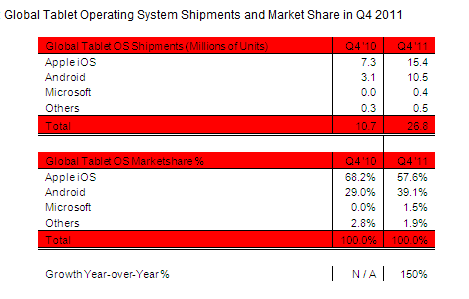
\includegraphics{images/QuarterlySales.png}
	\caption{Shipments refer to sell-in. Numbers are rounded. The definition of tablet does not include e-book readers.\cite{strategyanalytics}}
	\label{fig:QuarterlySales}
\end{figure}



Android is an open-source platform developed for mobile devices. The Android Open Source Project(AOSP) is maintained and further developed by the Open Handset Alliance(OHA), which is led by Google \cite{androidPhilosophy}. The companies from the OHA contributes to the project, these contributions are often made in form of engineering resources.

Android has a large community, spread over various websites, with different areas of expertise. This provides developers of android applications, with a community where they can find help with their nich� \cite{androidCommunity}.
Google, which is head of the android development, also has a website for teaching application developers how to program for the android platform \cite{androidDevelopers}. On Google�s website they also provide various tutorials, so one can easily get started developing for the android platform.

In this project we have been provided with several Samsung Galaxy Tablets 10.1 
\cite{tablet}. The firmware on the tablets is version 3.2\\

NOTE: Stod der ikke noget andet her? Jeg kan ikke finde det mere.

\section{Workform}


\chapter{Introduction}


% 
% common report
% 
\chapter{Initial Process}
In this chapter the problem definition for Oasis is described.
An analysis of the requirements, received from the other groups in the multi project, are performed and from the analysis the Oasis system architecture has been derived.

\section{Problem Definition}
\label{sec:OasisProblemDefinition}
In the multiproject a common problem definition have been stated, see Section \vref{sec:pdef}. The common problem definition is -- as stated -- to vouge for the individuel groups. Therefore we have devised a problem definition for Oasis.
It is as follows:

\begin{quotation}
	\textit{How can we provide a set of tools, which can help develop applications for the GIRAF system?}
\end{quotation}

\section{Requirements}
Before the development can begin the requirements for the software must be analysed.
The requirements stem from the multiproject groups and the contact persons.
Examples of the requirements received can be seen in Appendix \vref{sec:timerreq} and \vref{sec:customerReq}.

The derived informal requirements are:
\begin{itemize}
	\item Child profile handling
	\item Guardian profile handling
	\item Child and guardian relation handling
	\item Application specific profile setting handling
	\item Certificate handling
	\item Media handling
	\item Media access handling
	\item Media to media relation handling
	\item Department handling
	\item Department to subdepartment handling
	\item Profile to department relation handling
\end{itemize}

We have decided to develop a database and a library, which are to be used by GIRAF applications.
As an example of a GIRAF application, that uses the library and database, we will develop an administration application.

\section{System architecture}
\label{sec:OasisSystemArchitecture}
Oasis consists of three parts; The Oasis Local Db, the Oasis Lib, and the Oasis App. This is shown in Figure \vref{fig:systemArchitecture}.

The Oasis Lib handles application interaction with the Oasis Local Db, and every GIRAF application should be utilizing this library.
Another feature the Oasis Lib offers is the ability to handle synchronization between the Oasis Local Db and Savannah.

The last part is the Oasis App.
This application allows interaction with the Oasis Local Db through the Oasis Lib. 
Some of the features of the Oasis App are creation and removal of profiles and departments.
It also enables the user to handle relations between specific elements.

\begin{figure}
	\centering
		\includegraphics[width=\textwidth]{Images/Giraf_comp_pic_fixed}
	\caption{The GIRAF sytem architecture.}
	\label{fig:systemArchitecture}
\end{figure}
\section{System Definition}
The application we are developing is targeted for android tablets running Android 3.2. The use space is institutions and homes of autistic children.\\
   The application is meant as a tool, such that parents and educators can visualize time in a way customized for each child by changing color schemes, symbols, forms, and save this information in profiles stored on a server. The visualization is formed as a full-screen timer, which can be customized to be shown as an hour glass or a stop watch.\\
   Furthermore the guardians should be able to add pictograms to the timer view, to show them what they are going to do while the time is running, and what they are going to do when the time has run out.
   
\begin{comment}   
  In addition, the timer application should be used to control the allowed time spent on other applications, such as games. When the launcher is in autist mode, the timer application should be opened as an overlay whenever another application is opened. This overlay shows how much time is left, and when the time is up, it will lock the given application with a customized cooldown. Also the timer application should include a timelock, such that other applications are only available in specific time spans.
\end{comment}



\chapter{Development}


\chapter{Design}


\section{Vision}
Since the launcher had both a child-mode and a guardian-mode when we came with the initial design, this vision relies on the vision of the launcher project.\\ \\
	The initial idea of the WOMBAT system was a three-application tool to help educators illustrate time for the children they work with. One parts is the timer application as it is implemented, from which it is possible to run customized timers, such as an hourglass or a digital watch. This part should be available only from the guardian-mode.\\ \\
  The second part of the system is a timer overlay, which is launched when other applications, for example game applications, are launched through the GIRAF launcher. When such applications are launched through guardian mode, the user should be prompted to select if there is a time limit on the application, and what the limit should be. If a time limit is chosen, the given application, i.e. a game, is run with the timer overlay showing a custom timer with the time left.\\
	If the launcher is in child-mode, and the child opens some application, the timer overlay is run according to settings chosen in the third and last part of the WOMBAT system: the settings application. The overlay can be used if a child is only allowed to play a game for 30 minutes a day, then the overlay can be customized to show the child how long time is left of the allowed time. When the time is run out, the application is automatically closed.\\ \\
	The settings application is only available from the guardian-mode in the launcher, and from this application it is possible to customize which applications should be run with the timer overlay. Also it is possible to define how the overlay for every child should look like, and what should happen when the time limit has been reached. Also it is also possible to set constrains for the applications, such as time constrains, i.e. certain applications can only be opened in a different timespan on the day, or when a specific application has been run for 30 minutes straight, the application is closed and cannot be opened before a certain "cooldown" time.

\section{Use Cases}
A few use cases for each part of the vision.

\section{Paper Prototyping}
Paper prototypes has been a tool in the first iterations in the development process. The initial idea of the system design was drawn on paper, so that our contact person, Mette als Andreasen, could give us some feedback on the design, before we started programming. Furthermore it made it easier for us to program, when there was a specific design to work towards.\\

\textit{Der skal sikkert lidt kilder og forklaringer til, samt reference til vores papirprototyper i appendix}

\subsection{Metaphors}
To enhance usability and learn-ability, we have used metaphors on the buttons in the application. On the "Attach"-button, used to attach a second timer or one or two pictograms to the main timer, we have placed a paper-clip, which is known from the attach function in other programs, for example Microsoft Outlook Express.\\

\textit{Screenshot a vores metafor, og eventuelt en kilde til, hvorfor det er smart at bruge metaforer}
\chapter{Development Process}
As stated in chapter \ref{cha:project_management}, the development method used in this project is a modification of SCRUM, which means that the development evolve through sprints.

\section{Sprint Walk-through}
\textit{Backlogs og smaa forklaringer til hver, samt aendringer i produktet, og forventningerne hertil fra sprint til sprint.}
\chapter{Implementation}
\label{imp}
\textit{In the this chapter parts of the software will be presented. The Source Code associated with the software will be presented and described as well. The software is based on the previously analyzed design and calculations. So far it has been described how the model is supposed to work, and now the software implementation will be described in detail.}\\
\\
Some features of the PARRET application will be described first as the problem that spurred the feature and what solution we thought up. 
We will then describe our solution to the problem with code segments and what notes we might have to the feature before recommending what to read when exploring the problem further.\\

Figure \ref{fig:ClassUMLPARROTPDF} depicts the PARROT Project in an UML Diagram, showing the class associations .

\begin{figure}
	\centering
		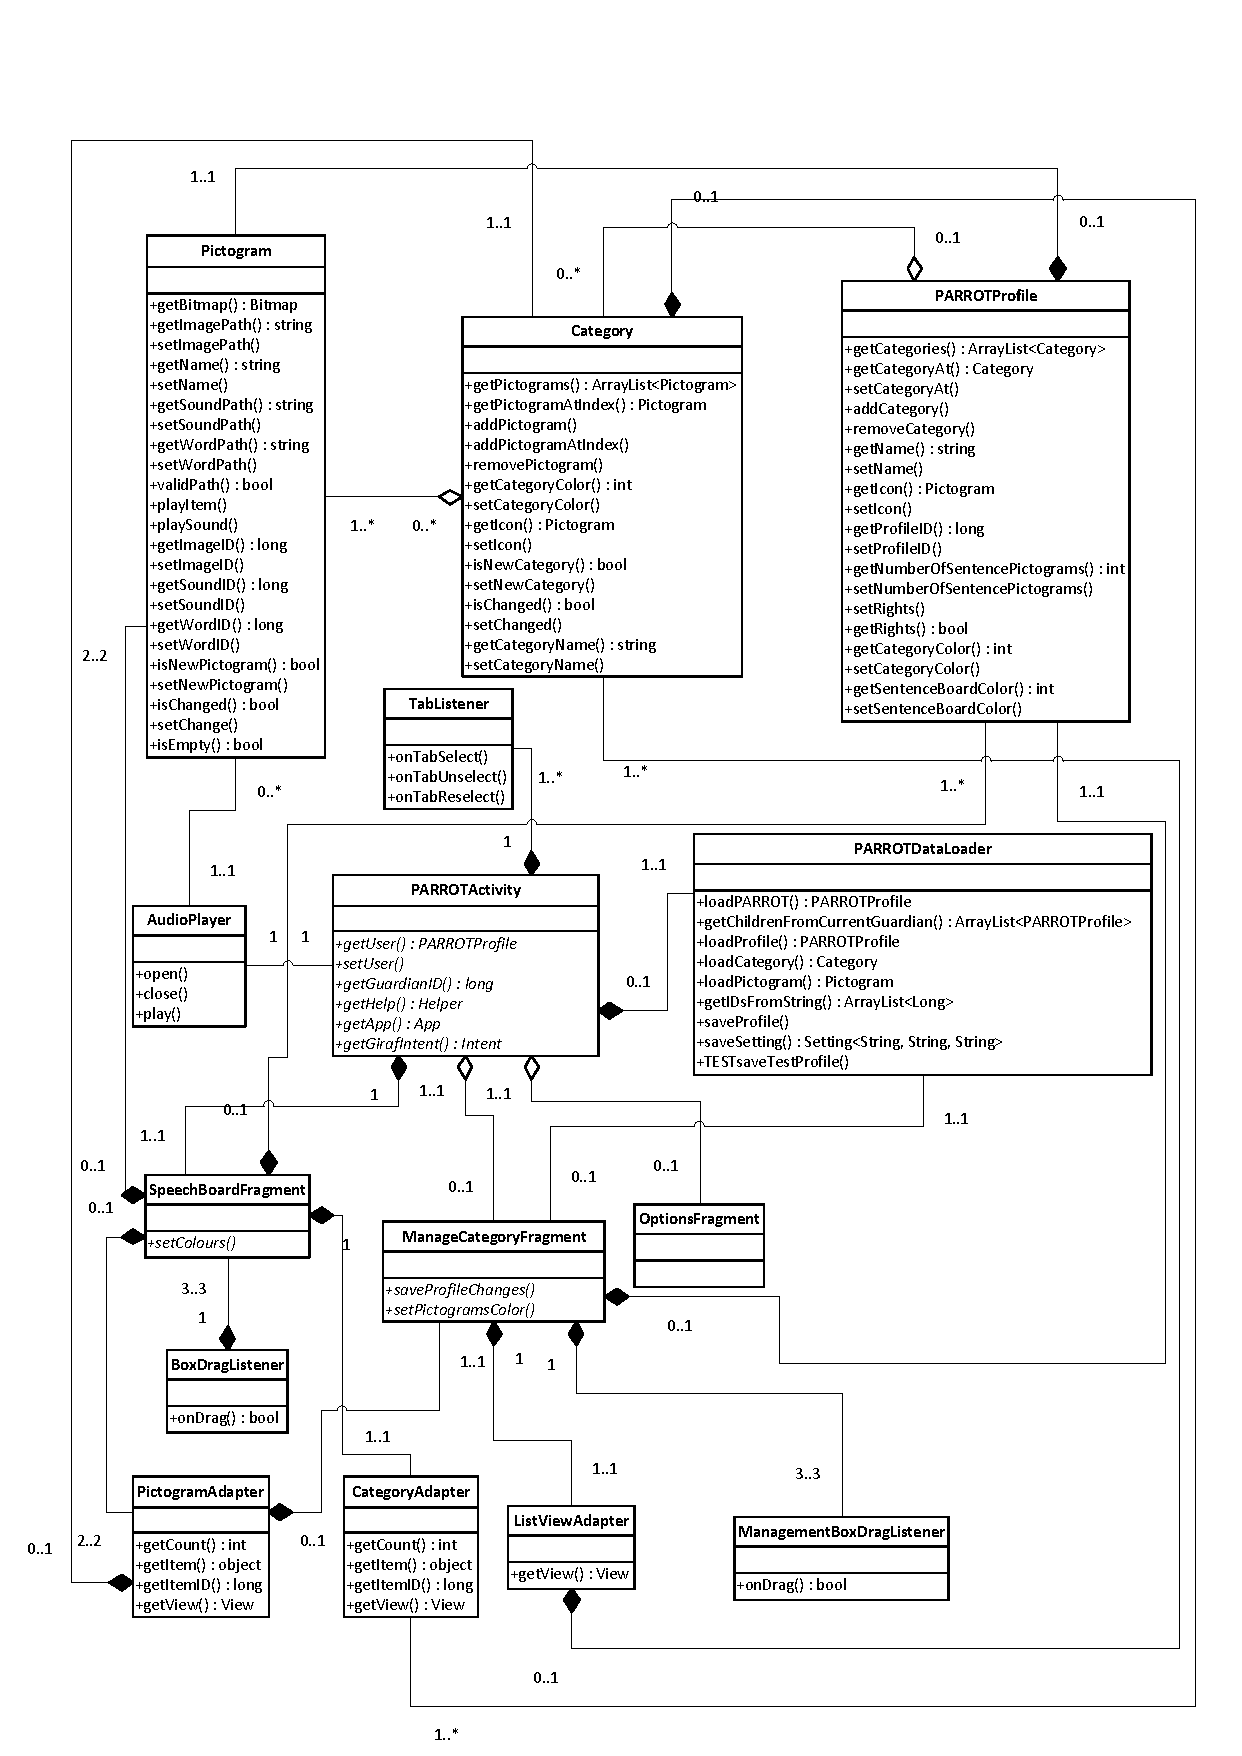
\includegraphics[width=1.0\textwidth]{input/images/ClassUMLPARROTPDF.pdf}
	\caption{UML Diagram of PARROT. Filled Diamonds are composition, Empty Diamonds are Aggregation.}
	\label{fig:ClassUMLPARROTPDF}
\end{figure}


\InputIfFileExists{input/Implementation/parrotxml}{}{}
\InputIfFileExists{input/Implementation/DragAndDrop}{}{}
\InputIfFileExists{input/Implementation/Sound}{}{}
\InputIfFileExists{input/Implementation/actionbar_tabs}{}{}
\InputIfFileExists{input/Implementation/Colour}{}{}
\InputIfFileExists{input/Implementation/Show_Pictograms}{}{}
\InputIfFileExists{input/Implementation/SentenceBoard}{}{}
\InputIfFileExists{input/Implementation/ManagingCategories}{}{}
\InputIfFileExists{input/Implementation/Database}{}{}\\
\\
\textit{The software for the PARROT application was presented in this chapter and the Source Code for the features and the design has been described. Now that the application is in a working state and running, it is possible to make the tests of the Source Code.}
\section{Test Cases}
\label{sec:test_cases}

\begin{center}
	\line(1,0){384}
\end{center}
\paragraph{Identifier}
	\textit{saveAs\#1}
\paragraph{Test item}
	Functionality to save customized timers in specific lists.
\paragraph{Input spec.}
	\begin{enumerate}
		\item Click "New Template", choose a timer type, click "Save As", and choose name and location. Check if the profile was saved in the chosen location and with the chosen name.
		\item Choose any configuration, edit the settings, click "Save As", and choose name and location. Check if the profile was saved in the chosen location and with the chosen name.
		\item Create a new configuration with random settings and use "Save As" to save it. Go to the saved configuration, and check if the settings has changed since the save.
		\item Choose an existing configuration or create a new one, and do step 1. with "Predefined" and "Last Used" as save locations.
		\item Do step 1-3 again, but clear the tablet memory before the correctness is checked.
	\end{enumerate}
\paragraph{Output spec.}
	\begin{enumerate}
		\item Configurations is saved in the chosen locations, unless the chosen locations is "Predefined" or "Last Used".
		\item Configurations is saved with the chosen name.
		\item Configurations is saved with the chosen settings.
	\end{enumerate}
\paragraph{environmental needs}
	\begin{itemize}
		\item Tablet running Android 3.2.
		\item Timer application installed.
		\item OasisLocalDatabase installed.
		\item One staff member to perform the test.
	\end{itemize}
\begin{center}
	\line(1,0){384}
\end{center}

\paragraph{Identifier}
	\textit{save\#1}
\paragraph{Test item}
	Functionality to save customized or predefined timers in the highlighted child, without having to choose name and location.
\paragraph{Input spec.}
	\begin{enumerate}
		\item Check if it is possible to save configurations in "Predefined" or "Last Used" by choosing one of the configurations in each list, edit some settings, and press "Save".
		\item Select a child, edit the settings, and press "Save". Check if the chosen settings were saved.
		\item Select a child, select a configuration among the child's configurations, edit the settings, and press "Save". Check if the chosen settings were saved in the same configuration.
		\item Select a child, edit the settings, and press "Save" two times and see if two identical configurations are saved on the given child.
		\item Highlight another configuration than the one you have just saved, then highlight the one you just saved and press "Save". Check if there is now saved a duplicate of the first saved configuration.
		\item Do step 2-3 again and check if any other configuration was changed during the saving process.
	\end{enumerate}
\paragraph{Output spec.}
	\begin{enumerate}
		\item Configurations is saved in the highlighted child.
		\item When "Predefined" or "Last Used" is highlighted, nothing is saved when the "Save" is pressed.
		\item New configurations are saved with the chosen settings.
		\item When selecting and saving existing configurations, they are updated with the edited settings.
	\end{enumerate}
\paragraph{environmental needs}
	\begin{itemize}
		\item Tablet running android 3.2.
		\item Timer application installed.
		\item OasisLocalDatabase installed.
		\item One staff member to perform the test.
	\end{itemize}
\begin{center}
	\line(1,0){384}
\end{center}

\paragraph{Identifier}
	\textit{checkLastUsed\#1}
\paragraph{Test item}
	Functionality to save timers into the "Last Used" list every any timer has been run.
\paragraph{Input spec.}
	\begin{enumerate}
		\item Run 3 different timers, and see if they were saved on top if the "Last Used" list.
		\item Repeat step 1, but clear the tablet memory before "Last Used" is inspected.
	\end{enumerate}
\paragraph{Output spec.}
	\begin{enumerate}
		\item Whenever a timer has been used, it is saved on top of the "Last Used" list.
	\end{enumerate}
\paragraph{environmental needs}
	\begin{itemize}
		\item Tablet running android 3.2.
		\item Timer application installed.
		\item OasisLocalDatabase installed.
		\item One staff member to perform the test.
	\end{itemize}
\begin{center}
	\line(1,0){384}
\end{center}

\paragraph{Identifier}
	\textit{hOnClick\#1}
\paragraph{Test item}
	Functionality to highlight list items when they are clicked.
\paragraph{Input spec.}
	\begin{enumerate}
		\item Select three different list items in both the child list and the configuration list and see if they stay highlighted.
	\end{enumerate}
\paragraph{Output spec.}
	\begin{enumerate}
		\item When a list item is selected, it is highlighted, and it stays highlighted until another list item is selected.
	\end{enumerate}
\paragraph{environmental needs}
	\begin{itemize}
		\item Tablet running android 3.2.
		\item Timer application installed.
		\item One staff member to perform the test.
	\end{itemize}
\paragraph{Special procedural requirements}
	\begin{itemize}
		\item The configurations on every child will always be visible when a child list has been selected. Therefore, make sure that the highlighted child has at least one configuration before testing.
		\item There is no element in the configuration list if no element in the child list has been selected.
	\end{itemize}
\begin{center}
	\line(1,0){384}
\end{center}

\paragraph{Identifier}
	\textit{stillHAfterSave\#1}
\paragraph{Test item}
	Functionality to highlight list items after a save procedure.
\paragraph{Input spec.}
	\begin{enumerate}
		\item Select a child and a configuration, edit the settings for the configuration, and click "Save". See if the selected list items stay highlighted after it has been updated.
	\end{enumerate}
\paragraph{Output spec.}
	\begin{enumerate}
		\item When a child and configuration is selected, and the settings for that configuration is changed and saved, the child list item and configuration list item is still highlighted.
	\end{enumerate}
\paragraph{environmental needs}
	\begin{itemize}
		\item Tablet running android 3.2.
		\item Timer application installed.
		\item One staff member to perform the test.
	\end{itemize}
\paragraph{Special procedural requirements}
	\begin{itemize}
		\item The configurations on every child will always be visible when a child list has been selected. Therefore, make sure that the highlighted child has at least one configuration in the list before testing.
		\item There is no element in the configuration list if no element in the child list has been selected.
		\item When a configuration is selected, the settings for that configuration is always shown set in the "Customize" menu.
	\end{itemize}
\paragraph{Intercase dependencies}
	\textit{save\#1}
\begin{center}
	\line(1,0){384}
\end{center}

\paragraph{Identifier}
	\textit{hChildOnLaunch\#1}
\paragraph{Test item}
	Functionality to highlight list items according to the chosen child when the application is launched through the GIRAF launcher.
\paragraph{Input spec.}
	\begin{enumerate}
		\item Start the GIRAF launcher and open the timer application.
		\item Select a child and note the name of the child.
	\end{enumerate}
\paragraph{Output spec.}
	\begin{enumerate}
		\item The child selected in the GIRAF launcher is highlighted and the configurations belonging to this child is loaded.
	\end{enumerate}
\paragraph{environmental needs}
	\begin{itemize}
		\item Tablet running android 3.2.
		\item Timer application installed.
		\item GIRAF launcher installed.
		\item One staff member to perform the test.
	\end{itemize}
\paragraph{Special procedural requirements}
	\begin{itemize}
		\item The configurations on every child will always be visible when a child list has been selected. Therefore, make sure that the highlighted child has at least one configuration before testing.
		\item There is no element in the configuration list if no element in the child list has been selected.
	\end{itemize}
\begin{center}
	\line(1,0){384}
\end{center}

\paragraph{Identifier}
	\textit{checkTimerTime\#1}
\paragraph{Test item}
	Functionality which draws and updates the timer according to the time left and ensures the timer ends when the time is up.
\paragraph{Input spec.}
	\begin{enumerate}
		\item Run four different timer styles with a static timespan (fx 20 minutes).
		\item Each time a timer is started, start a precise independent stopwatch.
		\item When the timer reaches zero stop the independent stopwatch.
	\end{enumerate}
\paragraph{Output spec.}
	\begin{enumerate}
		\item The stopwatch must deviate no more than two seconds from the time selected in \textbf{input spec.} step [1].
	\end{enumerate}
\paragraph{environmental needs}
	\begin{itemize}
		\item Tablet running android 3.2.
		\item Timer application installed.
		\item Stopwatch.
		\item One staff member to perform the test.
	\end{itemize}
\begin{center}
	\line(1,0){384}
\end{center}

\paragraph{Identifier}
	\textit{checkDoneFunc\#1}
\paragraph{Test item}
	The "Done" screen appearing when the time has run out.
\paragraph{Input spec.}
	\begin{enumerate}
		\item Start a timer at any timespan and let the time run out. See if the "Done" screen appears within two seconds after the time has run out.
		\item Start a timer at any timespan and click the "back" button, and wait at least the amount of time the timer would have run, to verify that the "Done" screen do not show up anyways, if the timer has been interrupted.
	\end{enumerate}
\paragraph{Output spec.}
	\begin{enumerate}
		\item When a timer has been run, and not interrupted, the "Done" screen appears about two seconds after the time has run out.
		\item The "Done" screen is only shown if the timer is not interrupted, and the time has run out.
	\end{enumerate}
\paragraph{environmental needs}
	\begin{itemize}
		\item Tablet running android 3.2.
		\item Timer application installed.
		\item Stopwatch.
		\item One staff member to perform the test.
	\end{itemize}
\paragraph{Intercase dependencies}
	Test case: \textit{checkTimerTime\#1}
\begin{center}
	\line(1,0){384}
\end{center}



\chapter{Discussion}


\chapter{Reflections and Evaluations}
\textit{Hvordan har brugen af pair programming og refactoring fungeret\\
Hvordan har SCRUM fungeret som projekt styring\\
}
\section{Conclusion}
\textit{Konklusionen paa projektet}

\section{Future Work}
\textit{Port to handset\\
OpenGL timers\\
Remake of design (drawer with profiles etc.)\\
Remake gradient Button\\
Implementation af vision om overlay\\}

\chapter{Conclusion}

\textit{In this chapter, we will present the conclusion of the project.}\newline
\\
The problem definition states:
\begin{quote}
How can we ease the daily life for children with ASD and their guardians, while complying with the study regulation?
\end{quote}
\\
We have designed a product that should help ease the use of pictograms. 
PARROT should help organize and ease access and use of pictograms. This allows for many of these to be handled simultaneously, without the need of the many physical pictograms and their bulky folders as mentioned in the analysis.\newline
It also gives the functionality to play sound, which could help some of the children learn the spoken language while using the pictograms to communicate. 
The idea of handling pictograms digitally also opens opportunities otherwise not easily accessible for the guardians.
For instance, we can change PARROT's colors according to the needs of the individual child. This include the colors for the different categories as well as those of the speech board.
The guardian can modify the categories and organize them according to the needs of the child.\newline
Since we have developed an application based on the needs of a third party, have been part of a multi project, and have performed dynamic blackbox testing as well as whitebox usability testing, we have upheld the goals of the study regulation.\newline

The whole project have been part of a greater multi project with five groups participating. 
As such we have not made a individual product, but one that is part of a greater product, GIRAF.  
GIRAF is not yet finished, but is hopefully going to be continued by other students on future semesters, so that it can become a product worthy of being used in the aforementioned institutions.\newline
As part of the multi project we have been using an agile development method, SCRUM.
Using SCRUM we have not spent the start of the semester analyzing the whole system, and designing it from the start. Instead we have analyzed and designed parts of the system one sprint at the time.
In previous semesters, we have wasted time on analyzing functionality that was never written, which was not the case in this semester.\newline
\\
\textit{This chapter presented the conclusion.}
\section{Future Work}

A number of tasks did not get completed in this semester. As this project is properly going to be continued by others students, it is not that big of a problem. 

\subsection{Server syncronization}
One of the main things which did not get completet, due to when the component we needed was available, we did not have more time to implement it, was the syncronization with the server. This can be implemented by using the components which the server group made. This would also make the sync status component in the launcher work.
Another improvement which could be implemented in a future continuation of the project, is the ability to syncronize images on the device, and update the paths dynamically.

\subsection{Unit tests}
Unit testing is an essential part of the project. We did manage to do some unit tests, but for future work more unit tests could be made, and it should be an ongoing process instead of doing them at the end of the semester.
Test to fail, to insure the lib robust DAN!

\subsection{Certificates}
Certificates is one of the core elements in the launcher, and therefore it is also reflected in the Oasis library. A couple of features where not completed for the certificates. The first one, was the possibility to set a time limit on the certificate, so it would have to renew itself after fx. 7 days. This would make the system more secure, but would rely on the users printing out new QR-codes each week, and the Oasis library to generate new QR-codes each week as well.
Another feature which certificates could have made use of, is the possibility to have multiple certificates per user, this would make it possible to have a QR-code for each department a person is in, and thereby only have access to the children in the department in question.

\subsection{Oasis App}

Mere p\aa{} app, refactor


\subsection{Test af dbprovider}
Test suite til db provider




\clearpage{\thispagestyle{empty}\cleardoublepage}

% Appendix
\chapter{Appendix}
\section{Requirements from Wombat}
\label{sec:timerreq}
I beh\o{}ver ikke smide det ind i objekter, da vi har vi allerede lavet objekter til vores data. 
Hvis vi blot kan f\aa{} dataen i en eller anden form for array, er det helt fint.

Vi ved ikke helt hvad for noget data der skal gemmes i settings, men vi har forst\aa{}et p\aa{} Henrik at man selv kan definere det n\aa{}r man gemmer.
Template

Function template
Her skriver man funktionen skal kunne
Data
Her skriver man hvilken data man gerne vil modtage
Damer
Create

Funktion createAutistSettings
Lave multiple Settings der er forbundet til en Autist

Funktion createLastUsedGuardian
Lave LastUsed liste der er forbundet til en Guardian
Retrieve

Funktion retrieveGuardianAutists
Man skal kunne hente Guardian samt alle autister der er linket til denne guardian.
Data
Guardian
Navn p\aa{} guardian
Autister

Funktion retrieveAutistSettings
Man skal kunne hente en specifik autist.
Data
Autist
Navn p\aa{} autist
Settings p\aa{} autist

Funktion retrieveLastUsed
Hente LastUsed liste fra en guardian
Data
Guardian
LastUsed
Update

Funktion updateAutistSetting
Update setting p\aa{} en bestemt autist

Funktion updateLastUsedGuardian
Update en bestemt guardians LastLused 
Delete

Funktion deleteSettingAutist
Slette en setting for en bestemt autist
Funktion deleteLastUsedGuardian
Slette LastUsed liste p\aa{} en guardian

\chapter{Project Backlog}
\label{sec:projectBacklog}
Here is the full project backlog for the project.

\begin{figure}[H]
	\centering
		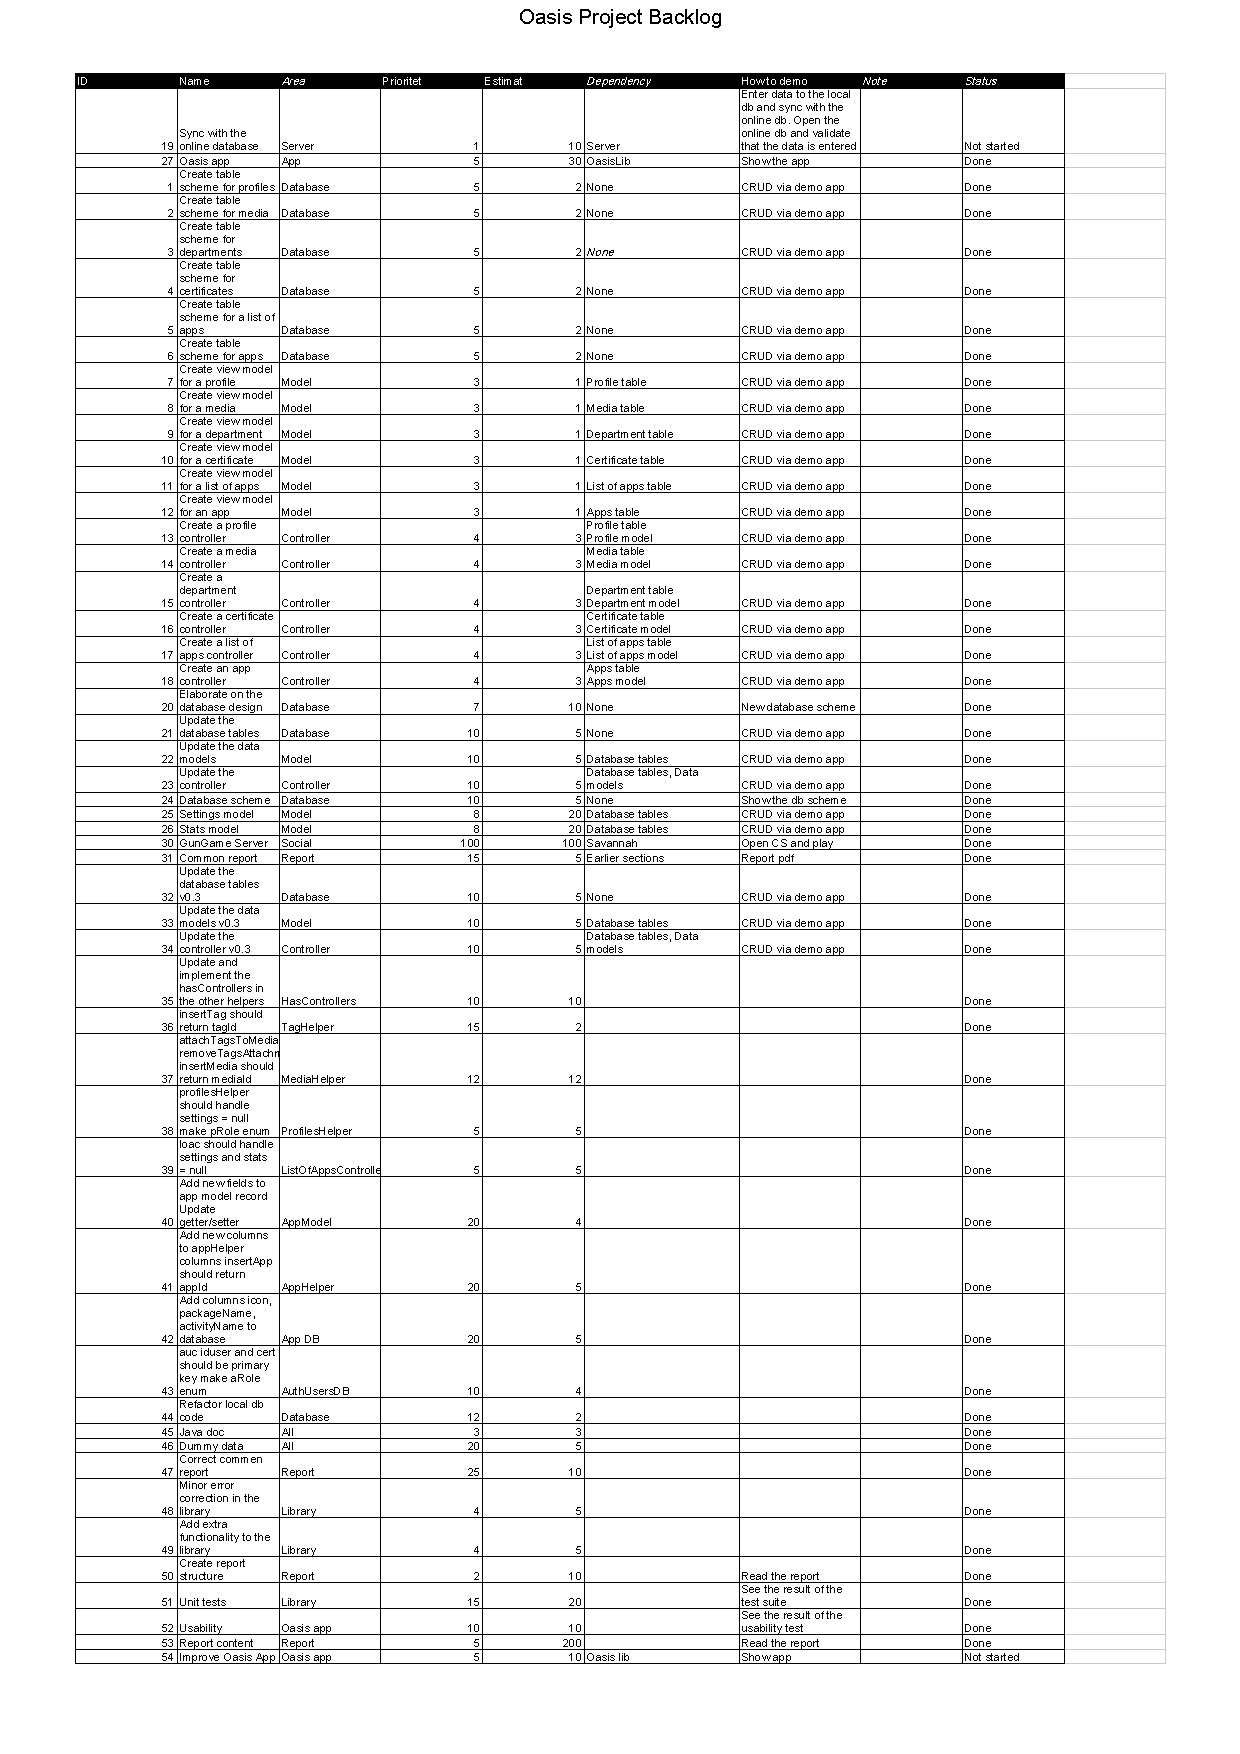
\includegraphics[width=\textwidth]{Images/OasisProjectBacklog}
	\caption{An overview of the Oasis project backlog.}
	\label{fig:projectBacklog}
\end{figure}

\chapter{Burndown Charts and Sprint Backlogs}
\label{sec:burn_back}
Here are an overview of all the sprints in this project.
	
\begin{figure}[H]
	\centering
		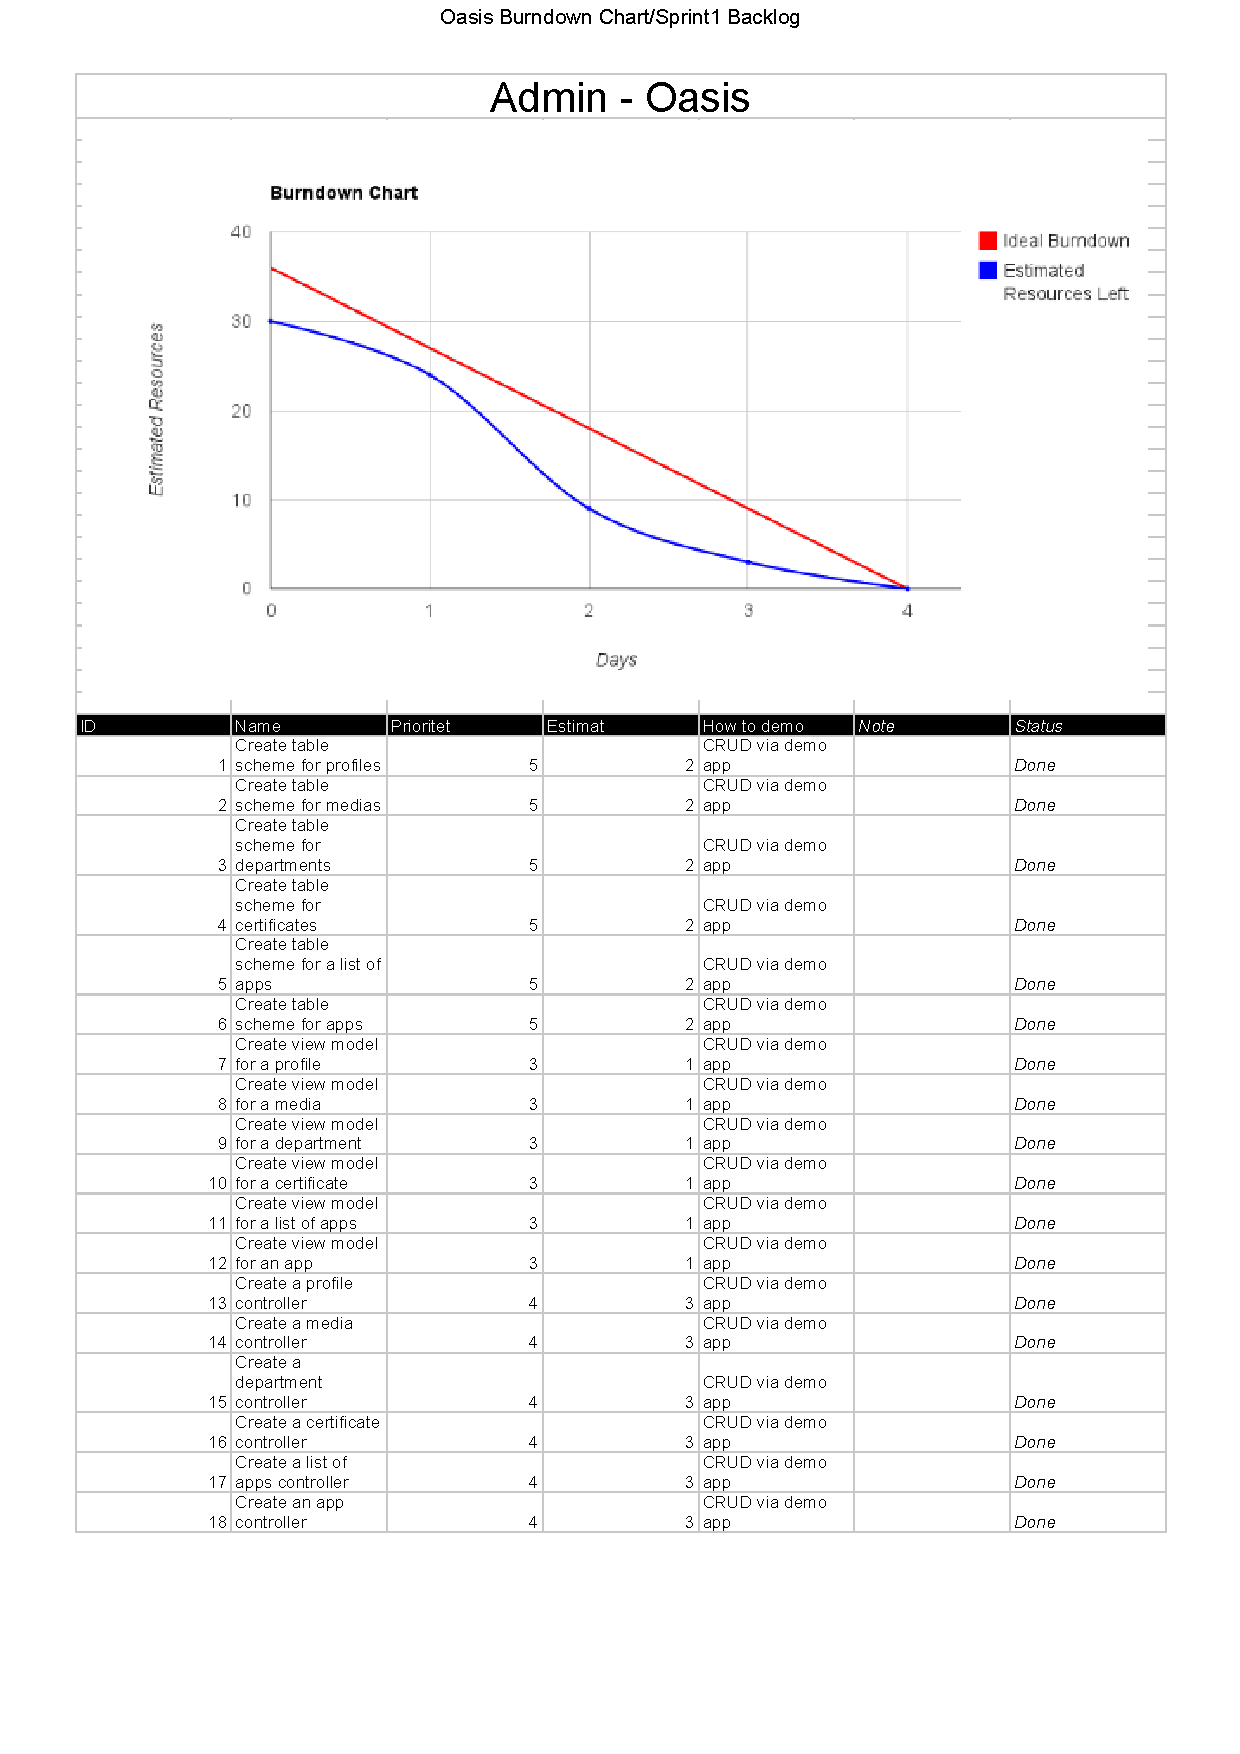
\includegraphics[width=\textwidth]{Images/sprint_backlogs/Oasis_Burndown_Chart_-_Sprint1_Backlog}
	\caption{The burndown chart and sprint backlog from sprint 1.}
	\label{fig:sprint1}
\end{figure}

\begin{figure}[H]
	\centering
		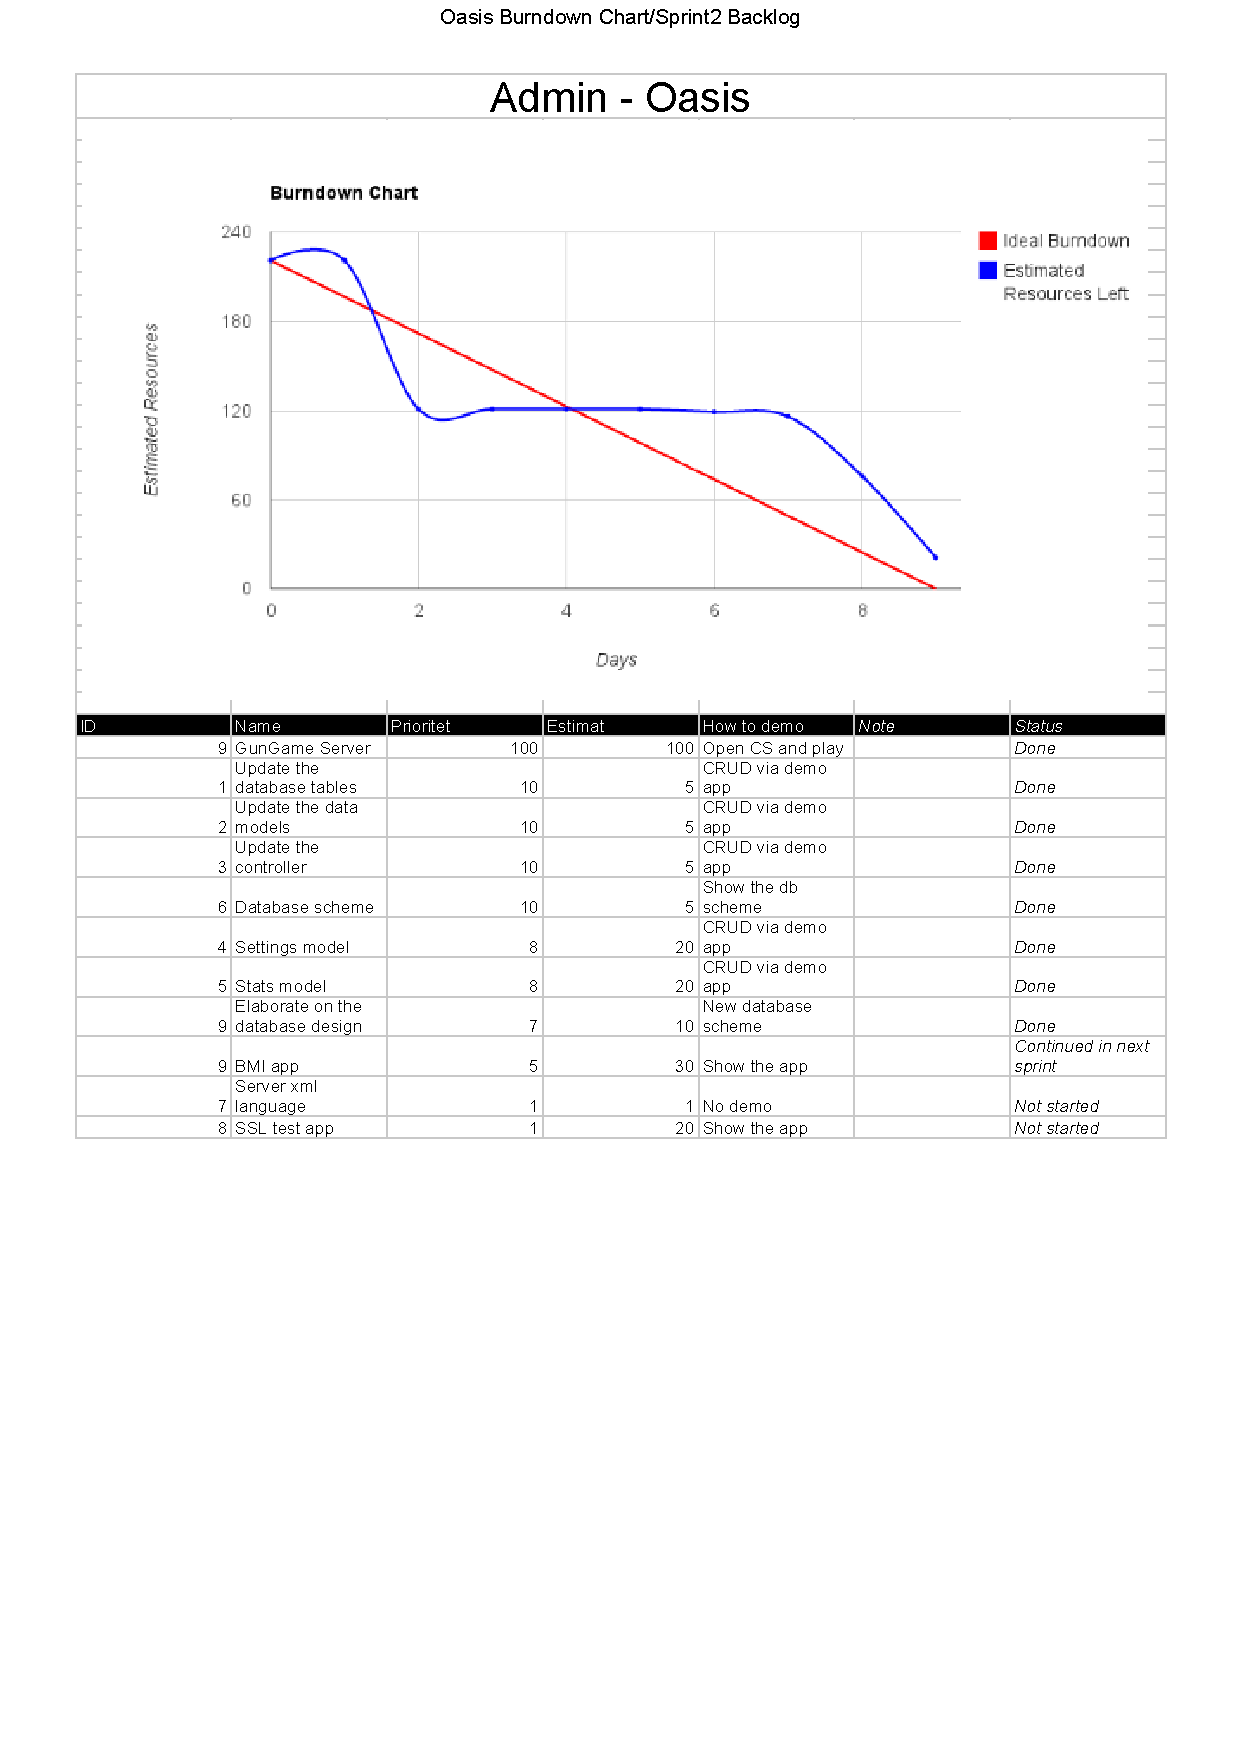
\includegraphics[width=\textwidth]{Images/sprint_backlogs/Oasis_Burndown_Chart_-_Sprint2_Backlog}
	\caption{The burndown chart and sprint backlog from sprint 2.}
	\label{fig:sprint2}
\end{figure}

\begin{figure}[H]
	\centering
		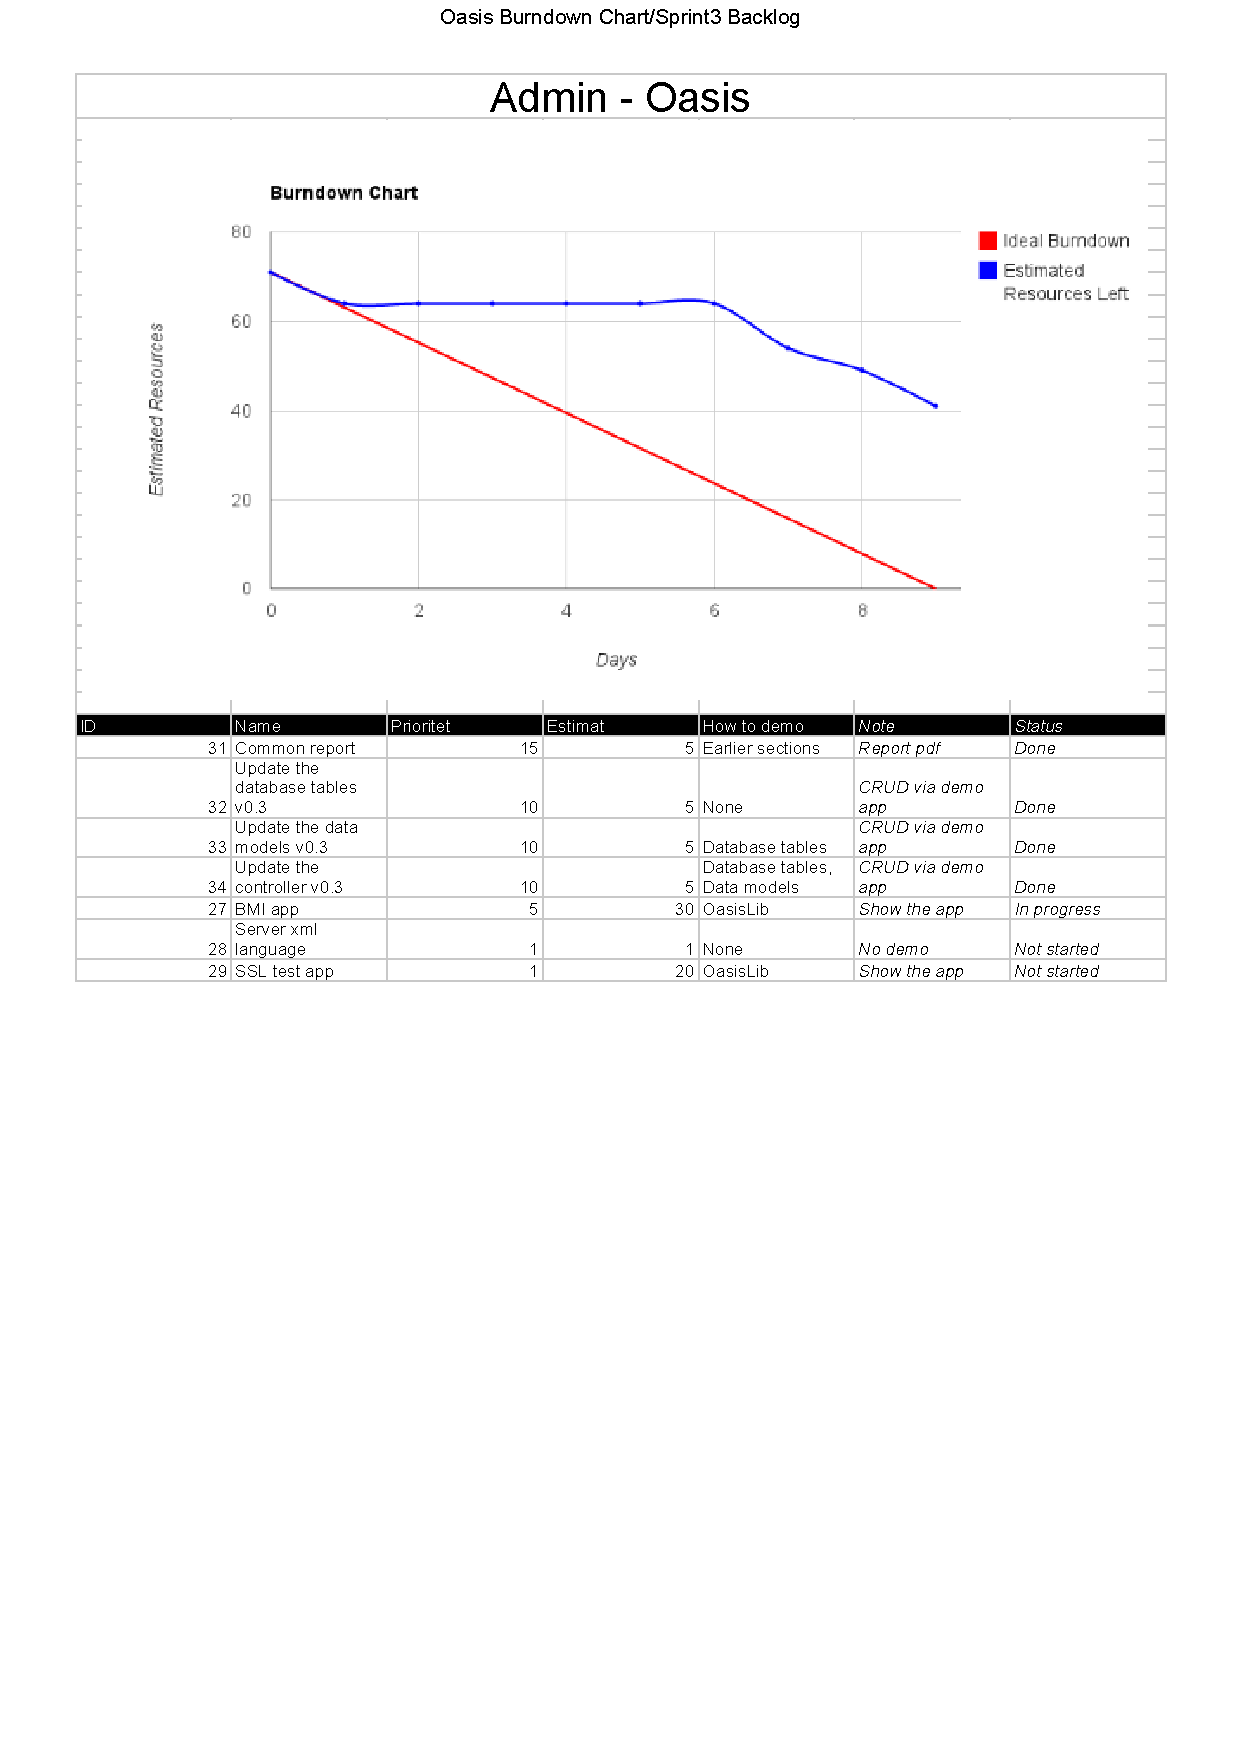
\includegraphics[width=\textwidth]{Images/sprint_backlogs/Oasis_Burndown_Chart_-_Sprint3_Backlog}
	\caption{The burndown chart and sprint backlog from sprint 3.}
	\label{fig:sprint3}
\end{figure}

\begin{figure}[H]
	\centering
		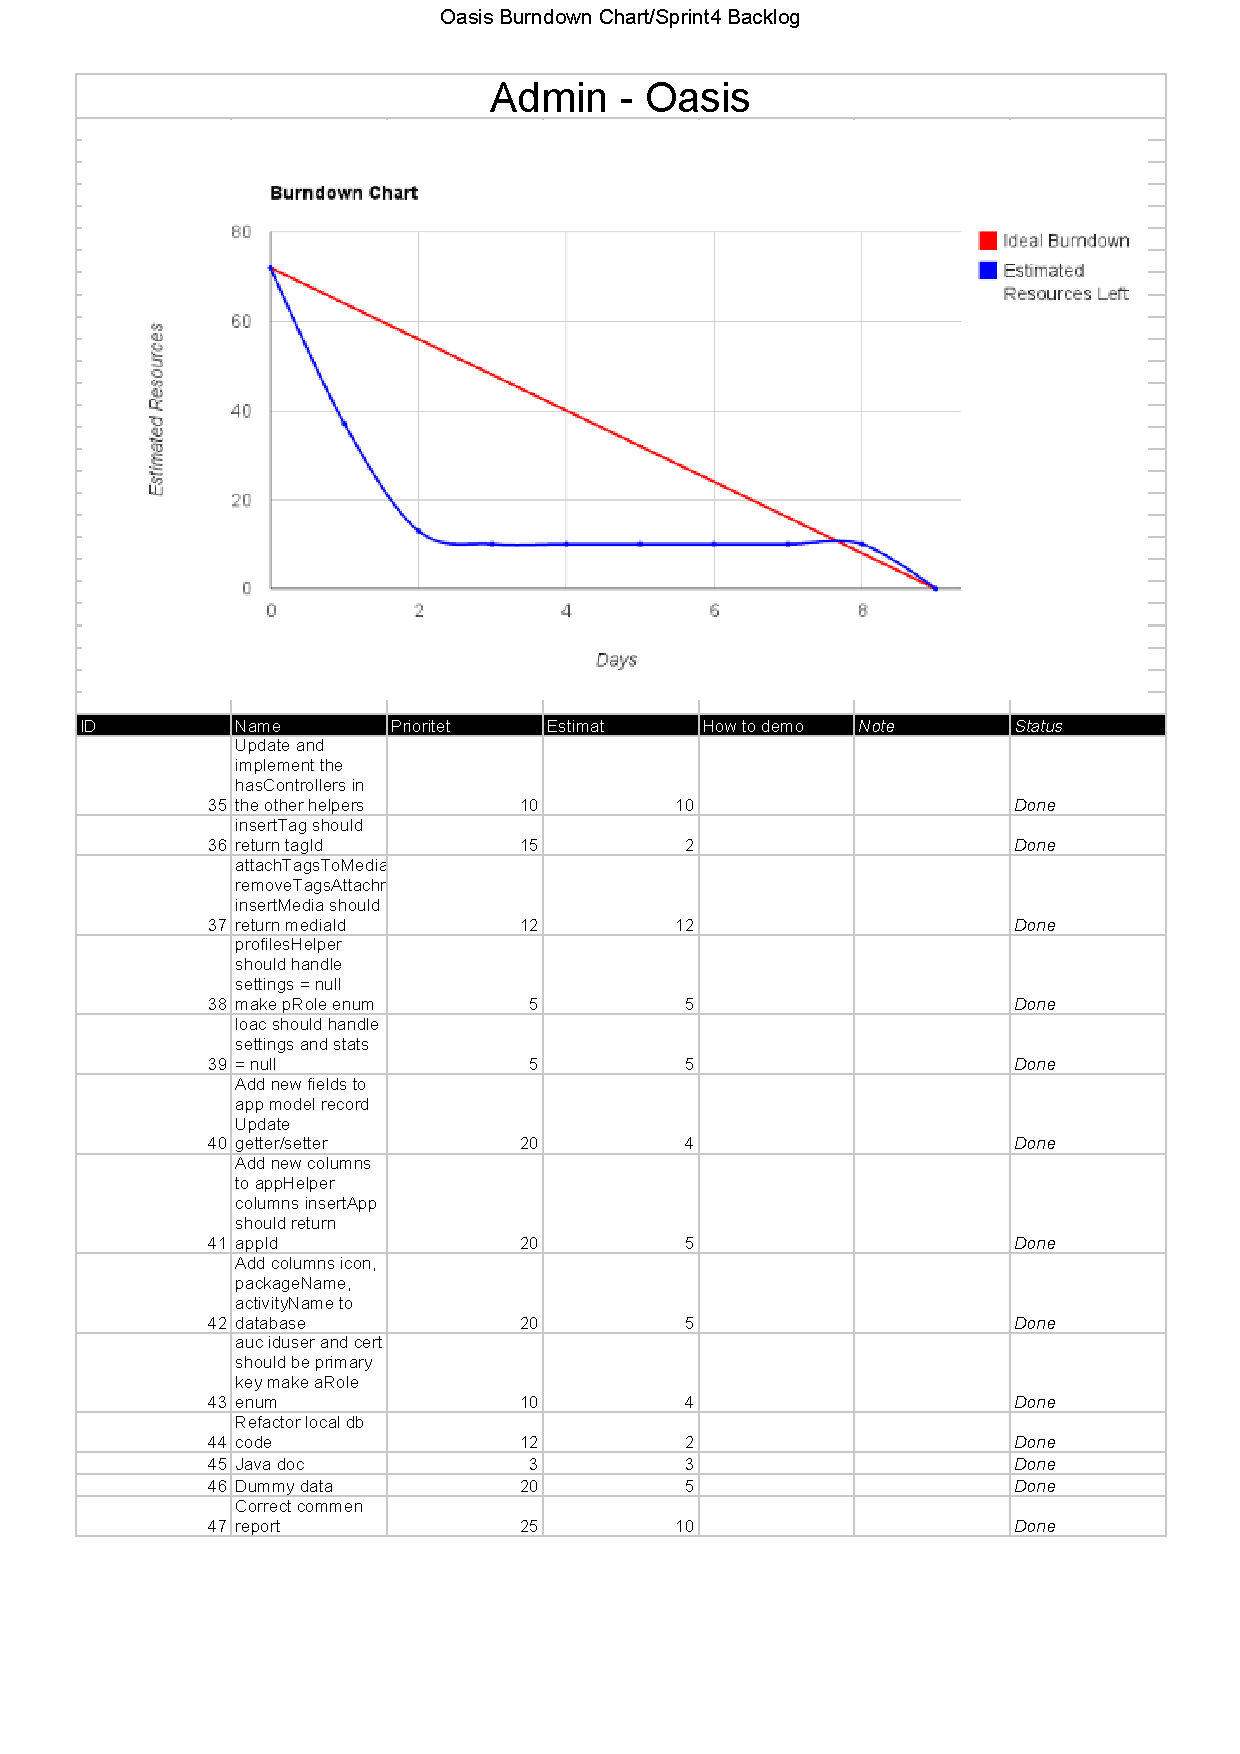
\includegraphics[width=\textwidth]{Images/sprint_backlogs/Oasis_Burndown_Chart_-_Sprint4_Backlog}
	\caption{The burndown chart and sprint backlog from sprint 4.}
	\label{fig:sprint4}
\end{figure}

\begin{figure}[H]
	\centering
		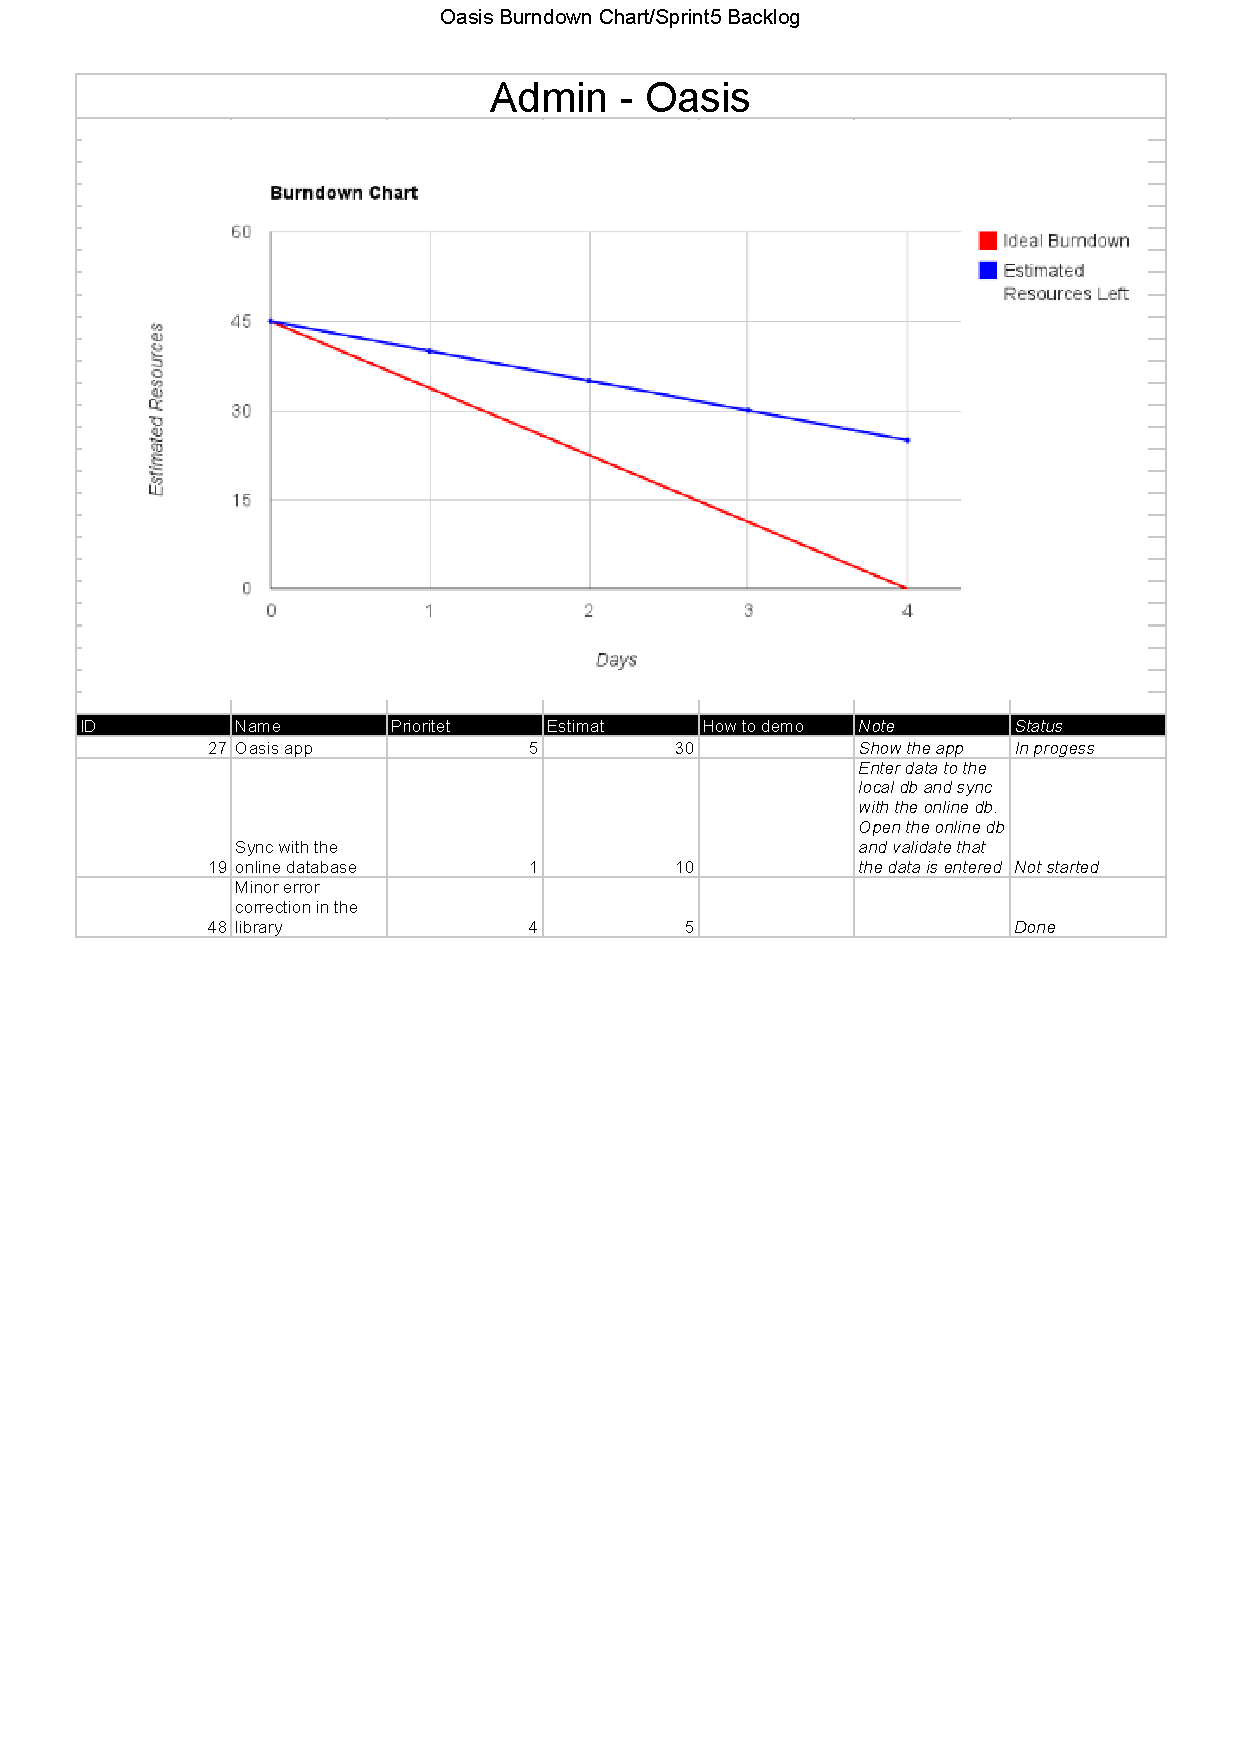
\includegraphics[width=\textwidth]{Images/sprint_backlogs/Oasis_Burndown_Chart_-_Sprint5_Backlog}
	\caption{The burndown chart and sprint backlog from sprint 5.}
	\label{fig:sprint5}
\end{figure}

\begin{figure}[H]
	\centering
		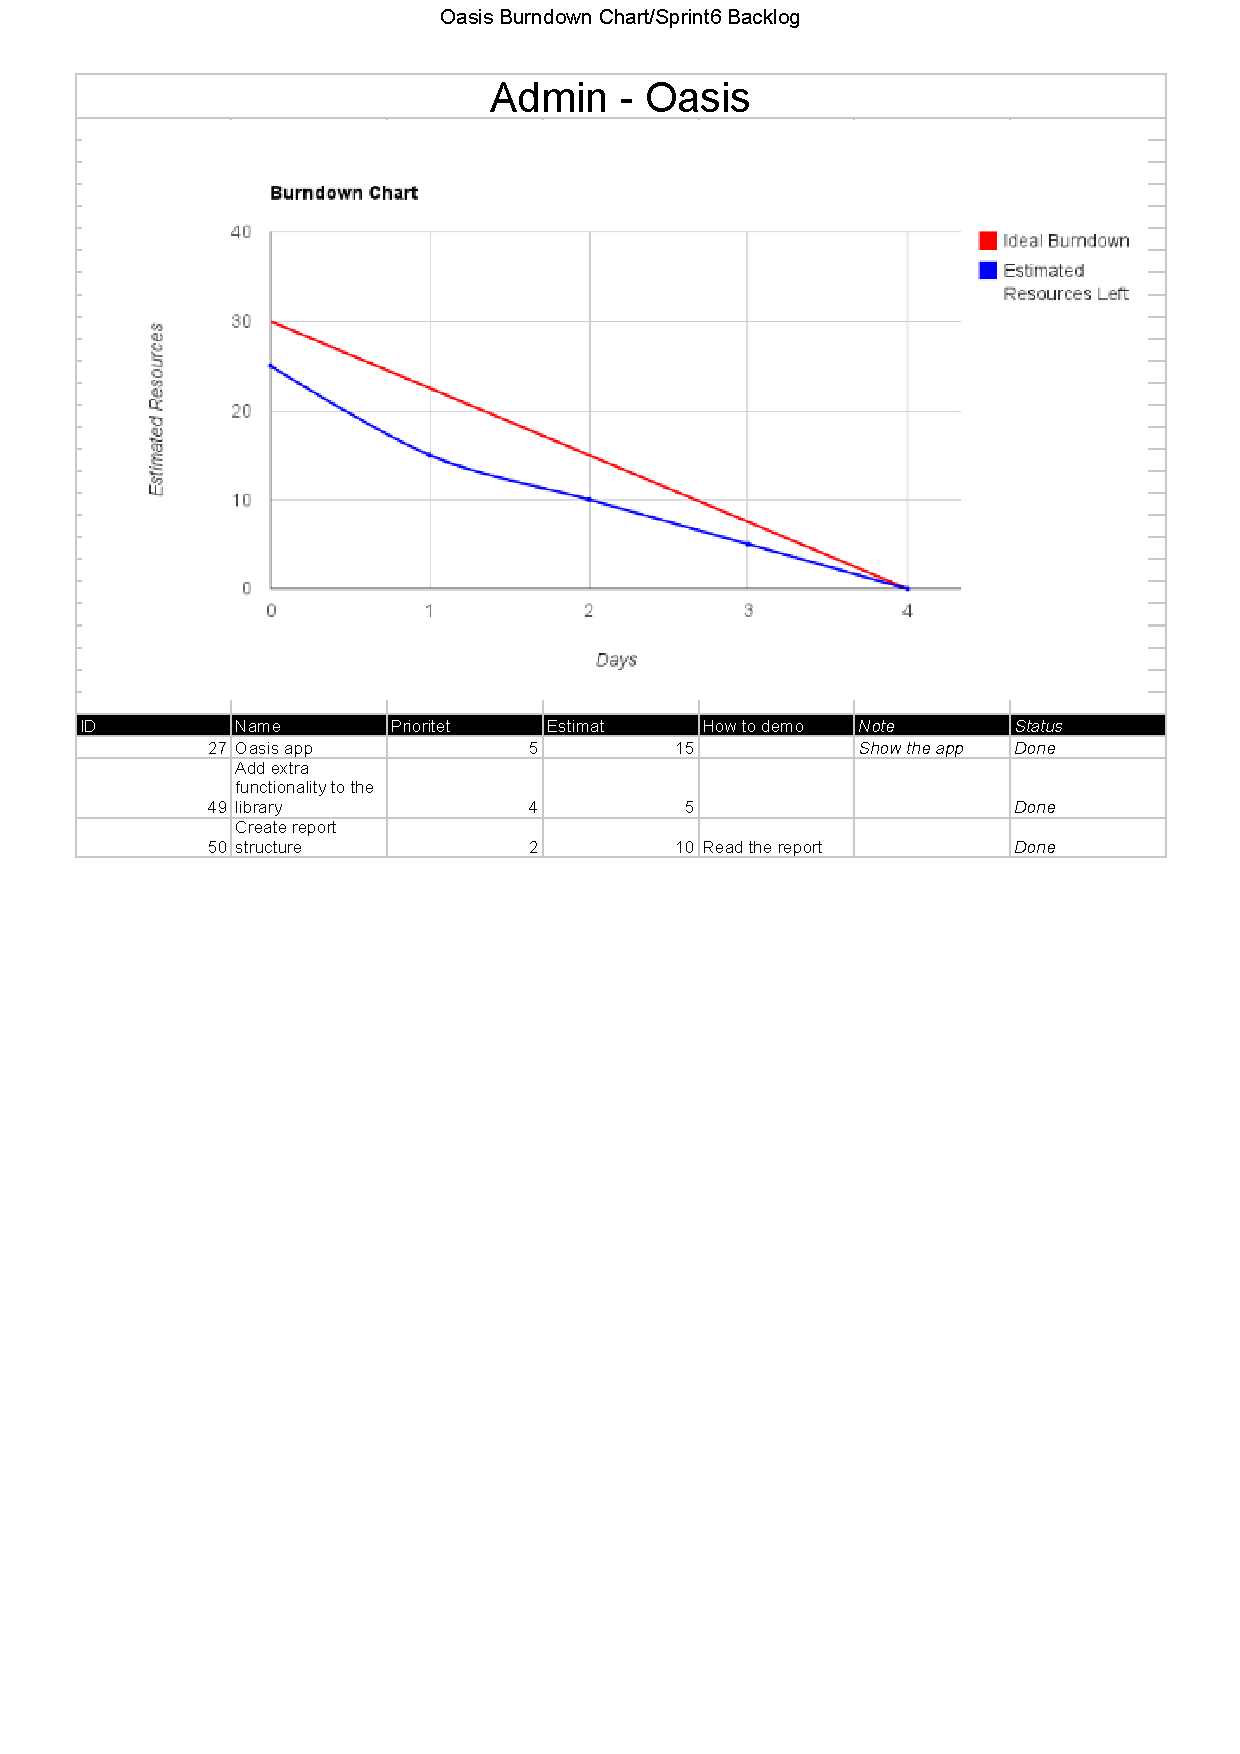
\includegraphics[width=\textwidth]{Images/sprint_backlogs/Oasis_Burndown_Chart_-_Sprint6_Backlog}
	\caption{The burndown chart and sprint backlog from sprint 6.}
	\label{fig:sprint6}
\end{figure}

\begin{figure}[H]
	\centering
		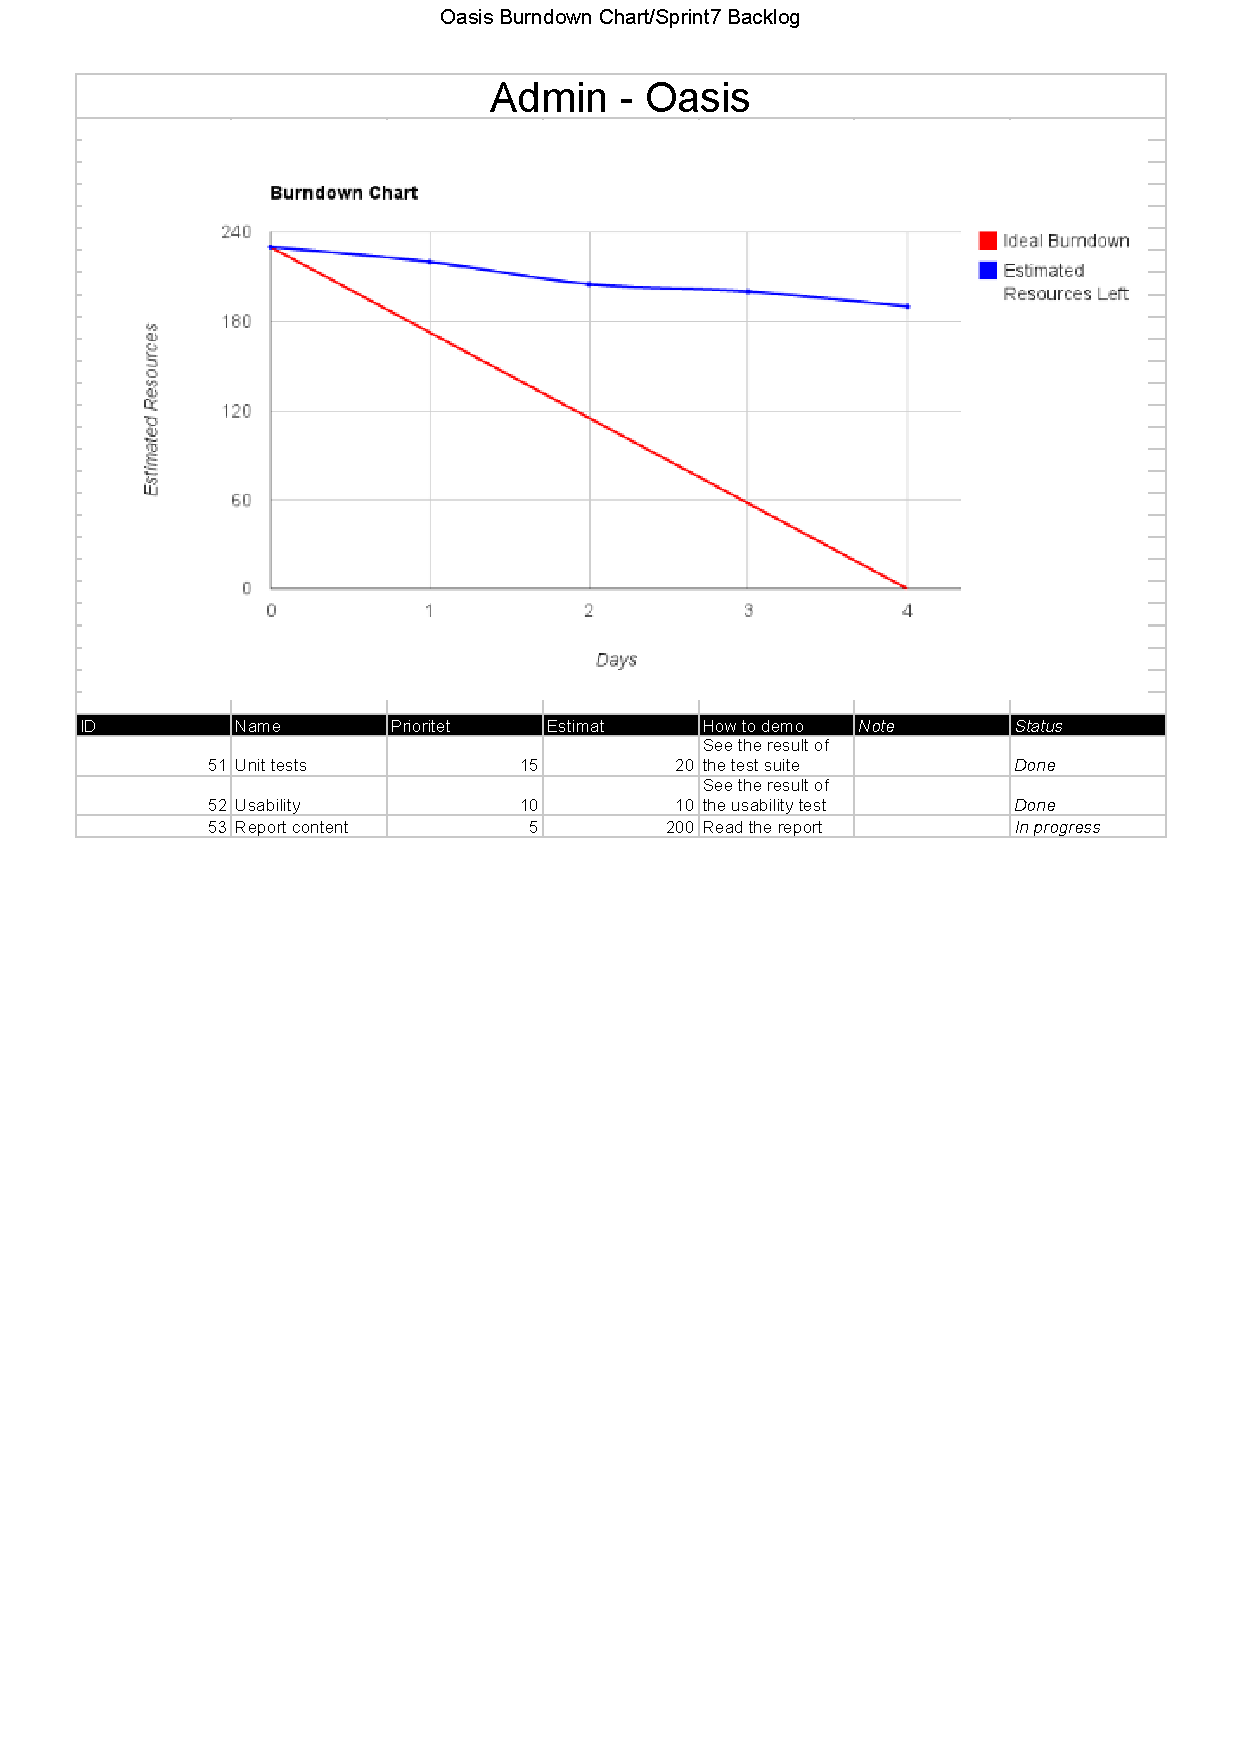
\includegraphics[width=\textwidth]{Images/sprint_backlogs/Oasis_Burndown_Chart_-_Sprint7_Backlog}
	\caption{The burndown chart and sprint backlog from sprint 7.}
	\label{fig:sprint7}
\end{figure}

\begin{figure}[H]
	\centering
		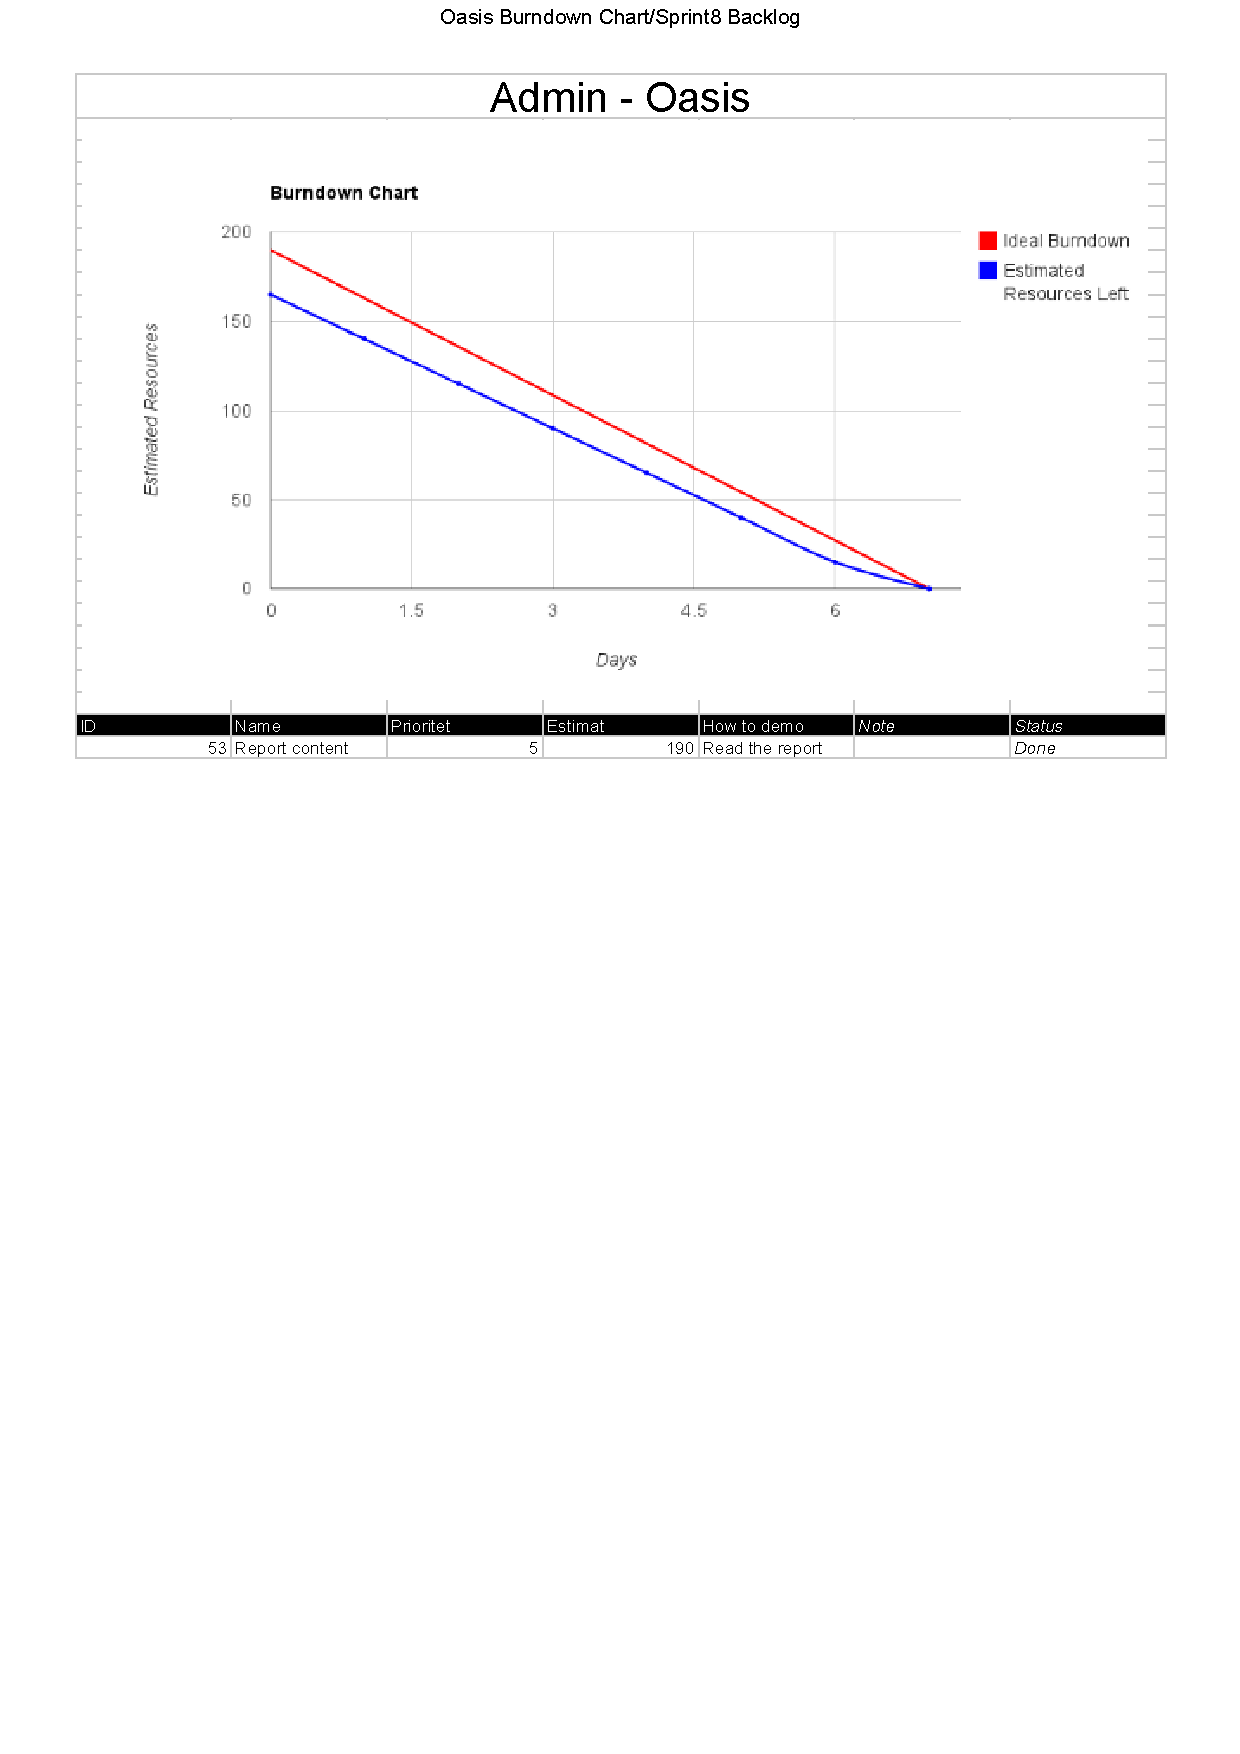
\includegraphics[width=\textwidth]{Images/sprint_backlogs/Oasis_Burndown_Chart_-_Sprint8_Backlog}
	\caption{The burndown chart and sprint backlog from sprint 8.}
	\label{fig:sprint8}
\end{figure}

\chapter{Change Log}
\label{sec:change_log}
Here is the full change log for the Oasis Library -- along with the models used in it -- and the Oasis Local Database.

\includepdf[width=\textwidth]{Images/OasisChangeLog}


\chapter{Mail correspondence with Customer}
\label{sec:customerReq}
\subsection{Mail To Customer}
Hej Kristine

Vi er blevet tildelt dig som kontakt person i forbindelse med vores projekt. Som n\ae{}vnt sidst s\aa{} arbejder vi p\aa{} at udvikle applikationer til android, som kan bruges enten af jer som p\ae{}dagoger og m\aa{}ske af autisterne p\aa{} sigt. Vi vil udvikle flere forskellige applikationer, og vi vil gerne l\o{}bende aftale m\o{}der med dig, hvor vi kan vise det samlede produkt som er lavet. P\aa{} den m\aa{}de kan vi f\aa{} feedback p\aa{} hvad der g\aa{}r godt og hvad der er knap s\aa{} godt.

Vores udviklings gruppe best\aa{}r af tre personer og vi skal lave en applikation der kan hj\ae{}lpe med at lave profiler der passer til b\o{}rnene. 

Da vi stadig kun er i gang med at planl\ae{}gge mener vi ikke at det er n\o{}dvendigt at holde et m\o{}de endnu. Men vi har nogen sp\o{}rgsm\aa{}l som vi gerne vil have dig til at svare p\aa{}:

\subsubsection{Hvilke informationer gemmer i omkring det enkelte barn?}
\begin{itemize}
	\item Journal nummer?
	\item Person nummer?
	\item Navn?
	\item Alder?
	\item S\ae{}rlige behov?
\end{itemize}

\subsubsection{a - Ur}
a1. Vil barnet kunne forst\aa{} at en hel cirkel kan have forskelligt tidsinterval?
a1.1 Eller er det bedst hvis cirklen har et fast tidsrum fx 1 time?
\\
a2. Hvis man skal m\aa{}le et tidsinterval p\aa{} uret, er det s\aa{} bedst at lade uret efterligne et almindeligt ur med 12 timer eller et stop-ur med kun 1 time?

\subsubsection{b - Timeglas}
b1. Vil barnet kunne forst\aa{} at det samme timeglas med den samme m\ae{}ngde sand kan varierer i tid?
\\
b2. Er det bedst at man varierer i m\ae{}ngden af sand i timeglasset eller at man varierer i timeglassets st\o{}rrelse?

\subsubsection{c - Aktivitetstid}
c1. Vil barnet kunne forst\aa{} at en linje der g\aa{}r hele vejen hen over sk\ae{}rmen kan varierer i tidsinterval?      
c1.1 Eller er det bedre hvis linjen har et fast tidsinterval og fx en halv linje derfor svarer til en halv time og en hel linje til en hel time? 

\subsubsection{d - Dagsplan}
d1. Hvis man laver en visuel dagsplan er det s\aa{} bedst at man laver et interval som viser tiden imellem to aktiviteter, eller at man viser alle aktiviter i l\o{}bet af dagen kombineret med en tidslinje?

\subsection{Mail From Customer}
Hej.
Tak for jeres mail.
Jeg skal besvare jeres mail s\aa{} godt som muligt, og s\aa{} m\aa{} i give lys hvis i har brug for at jeg uddyber.
\\
Vedr. informationer vedr. barnet:
Vi benytter et elektronisksystem som hedder, EKJ, hvor alle oplysninger p\aa{} b\o{}rnene er gemt. Det vil sige, pers. nr., adresse oplysninger, indbydelser, handleplaner og referater fra diverse m\o{}der.
 \\
UR: Hvis det er tydeligt vist at ``tiden g\aa{}r'' /skiven bliver mindre/forsvinder, som tiden g\aa{}r, vil barnet forst\aa{} meningen med uret. For at indikere forskellig tid, kan man benytte forskellige farvet baggrunde. Lilla:5 min. Gr\o{}n:10 min osv. Vi benytter kun kortere tidsintervaller,(1. min. 3. min. 5 min. -op til ca. 10-15. min) da 1 time er for abstrakt.
\\
Timeglas: Hvis der er en tydelig markering af tidsintervallet, som beskrevet ovenfor, er det muligt at bruge samme timeglas. Tror det vil give bedst forst\aa{}else for barnet, hvis m\ae{}ngden af sand varieres efter tid. 
\\
Aktivitetstid og dagsplan: (Tror J) Aktivitetstid kan bruges ved, at tiden bliver indikeret af m\ae{}ngden af aktiviteter.
 - Alts\aa{} 3-5 viste aktiviteter af gangen, og ikke s\aa{} meget om det er en time eller 15 min. 
Tiden kunne v\ae{}re en mulighed at tilf\o{}re, om n\o{}dvendigt. Mange af vores b\o{}rn har manglende fornemmelse for tid, og ofte har de brug for at se sm\aa{} konkrete sekvenser/beskeder frem for mange over l\ae{}ngere tid.
Derfor vil jeg tror de bedst kan overskue \textonehalf{} dag af gangen, men stadig have mulighed for at have dagen p\aa{} skemaet, hvor det kan vises i sekvenser.
\\
Jeg har samlet de to ovenst\aa{}ende punkter, da de nemt kommer til at gribe ind i hinanden.
Vores ugeskemaer i b\o{}rnehaven er vist med internationale farver, dem vil i ligeledes kunne benytte til at tydeligg\o{}re ugedagene.
Mandag: Gr\o{}n, Tirs.: Lilla, Ons.: orange, tors.: bl\aa{}, Fre.: gul, l\o{}r.: r\o{}d og s\o{}ndag: hvid.
\\
H\aa{}ber dette er uddybende nok, ellers m\aa{} i gerne skrive eller ringe til mig hvis det er nemmere.
\\
Ser  frem til at h\o{}rer fra jer igen.
\section{Notes from Interview}
\label{InterviewMette}
\textit{This is notes from an interview with Mette Als Andreasen, an educator at Birken in Langholt, Denmark.}

N�r tiden l�ber ud (kristian har tage et billede):\\
F�rdig - symbol\\
G� til skema - symbol\\
Taget fra boardmaker\\

Kunne v�re godt hvis man kunne s�tte egne billeder ind som start/stop symboler.\\


R�d farve $=$ nej, stop, aflyst.\\

De har s�dan et ur p� 60 minutter hvor tid tilbage er markeret med r�d, og s� bipper den lige kort n�r den er f�rdig.\\
  Det ville v�re fint hvis de kunne bruge sort/hvid til dem der ikke kan h�ndtere farver, men ogs� kan v�lge farver.\\

Stop-ur:\\
en fast timer p� 60 minutter $+$ en customizable som ikke ser helt magen til ud, som f.eks, kan v�re p� 5, 10 eller 15 minutter for en hel cirkel.\\

timeglas:\\
skift farve p� timeglassene, men ikke n�dvendigvis g�re dem st�rre. Kombinere med mere/mindre sand. Eventuelt kombinere med et lille digitalt ur, til dem der har brug for det, skal kunne sl�es til og fra.\\

Dags-plan:\\
ikke s�rlig relevant til de helt sm� og ikke s�rligt velfungerende b�rn. Men kunne v�re rigtig godt til de lidt �ldre.\\
   En plan g�r oppefra og ned, og hvis der s� skal specificeres noget ud til aktiviteterne, s� er det fra venstre mod h�jre ud fra det nedadg�ende skema.\\

Til parrot:\\
Godt med rigtige billeder af tingene, som p�dagogerne selv kan tage, eventuelt ogs� af aktiviteter, s� pedagogerne kan have billeder af aktiviter som de kan liste efter skeamet.\\

Der var mange skemaer rundt omkring, og der henviser det sidste billede i r�kken til n�ste skema, som h�nger f.eks. p� badev�relset eller i garderoben.

\chapter{Usability Documents}
\label{app:usability_documents}
\begin{figure}[H]
	\begin{center}
	
\includegraphics[width=\textwidth]{Appendix/invitation_to_usability_test.pdf}
	\end{center}
\caption{Invitation sent to the test persons of the usability test.}
\label{fig:usability_test_invitation}
\end{figure}

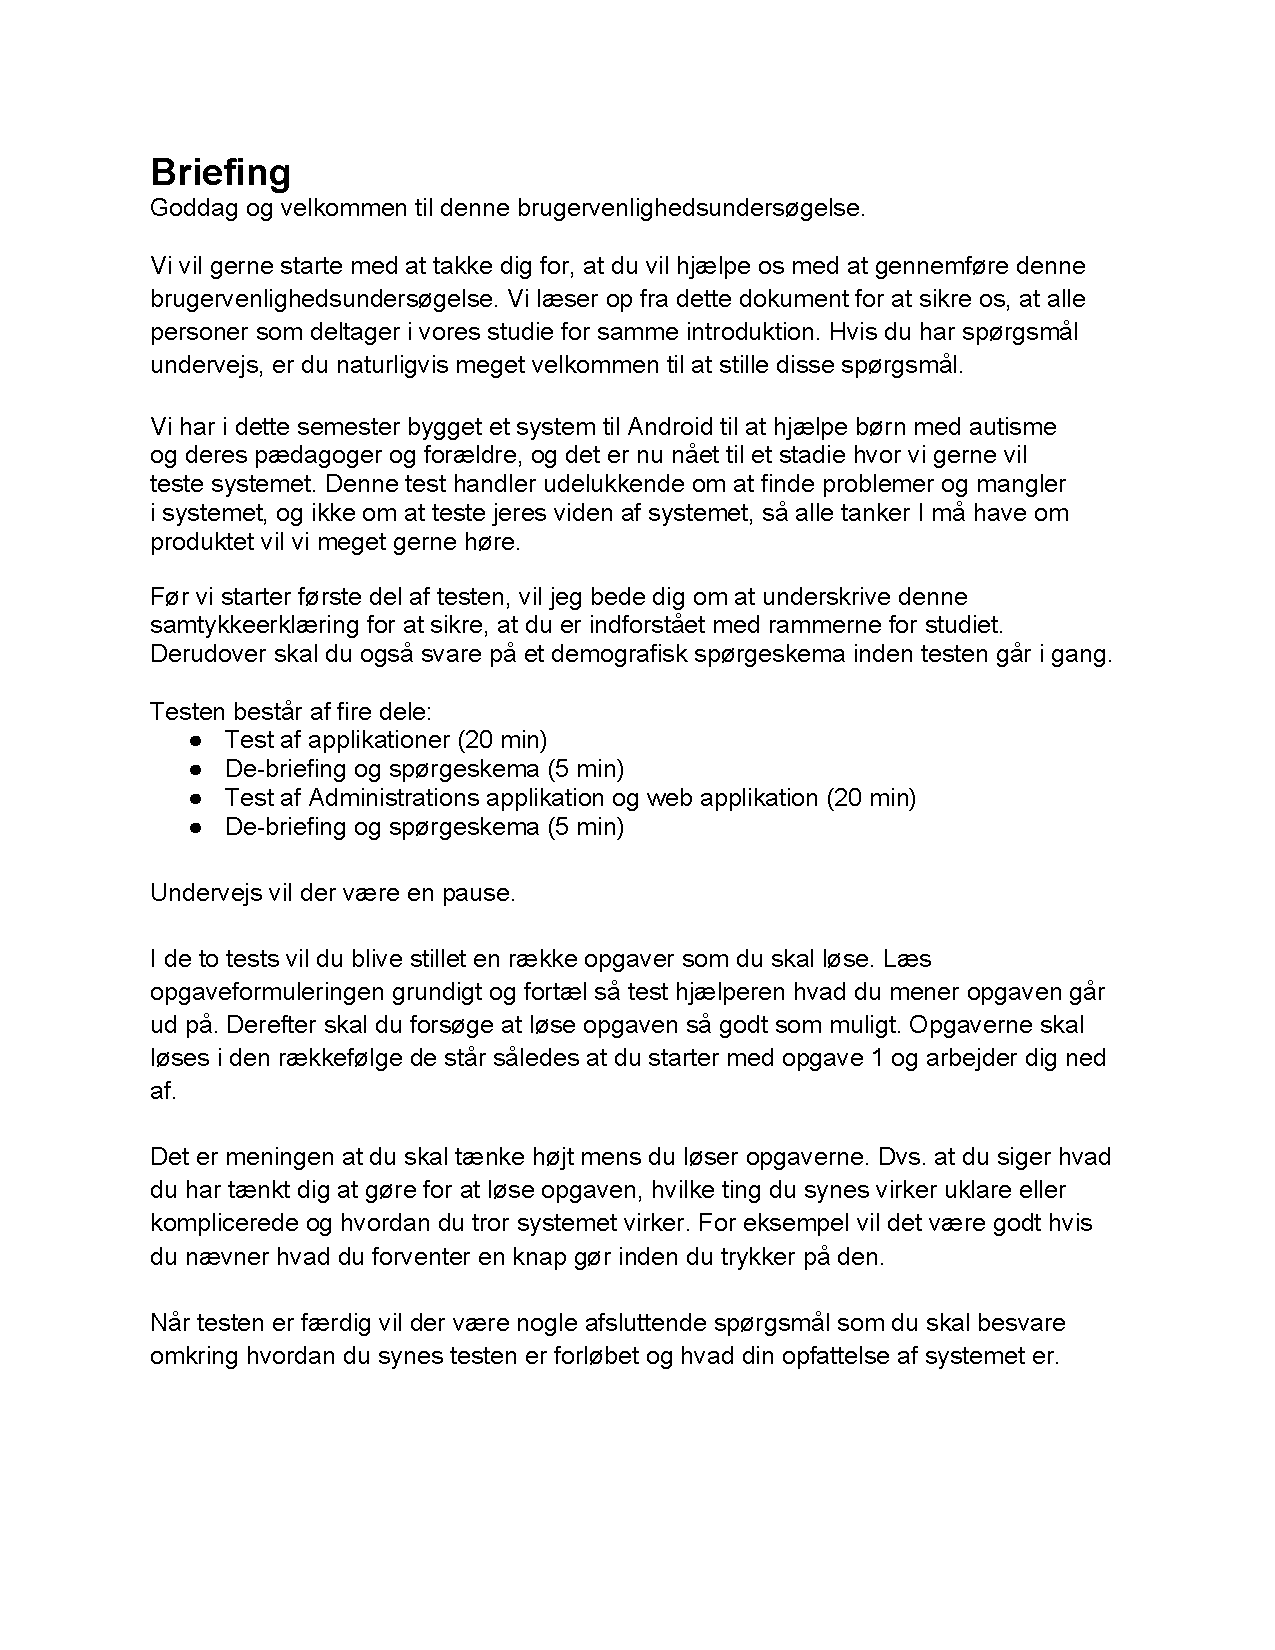
\includepdf{Appendix/Briefingogde-briefing}

\subsection{Questionnaires from usability}

\label{questionnaires}

\begin{figure}[h]
	\centering
		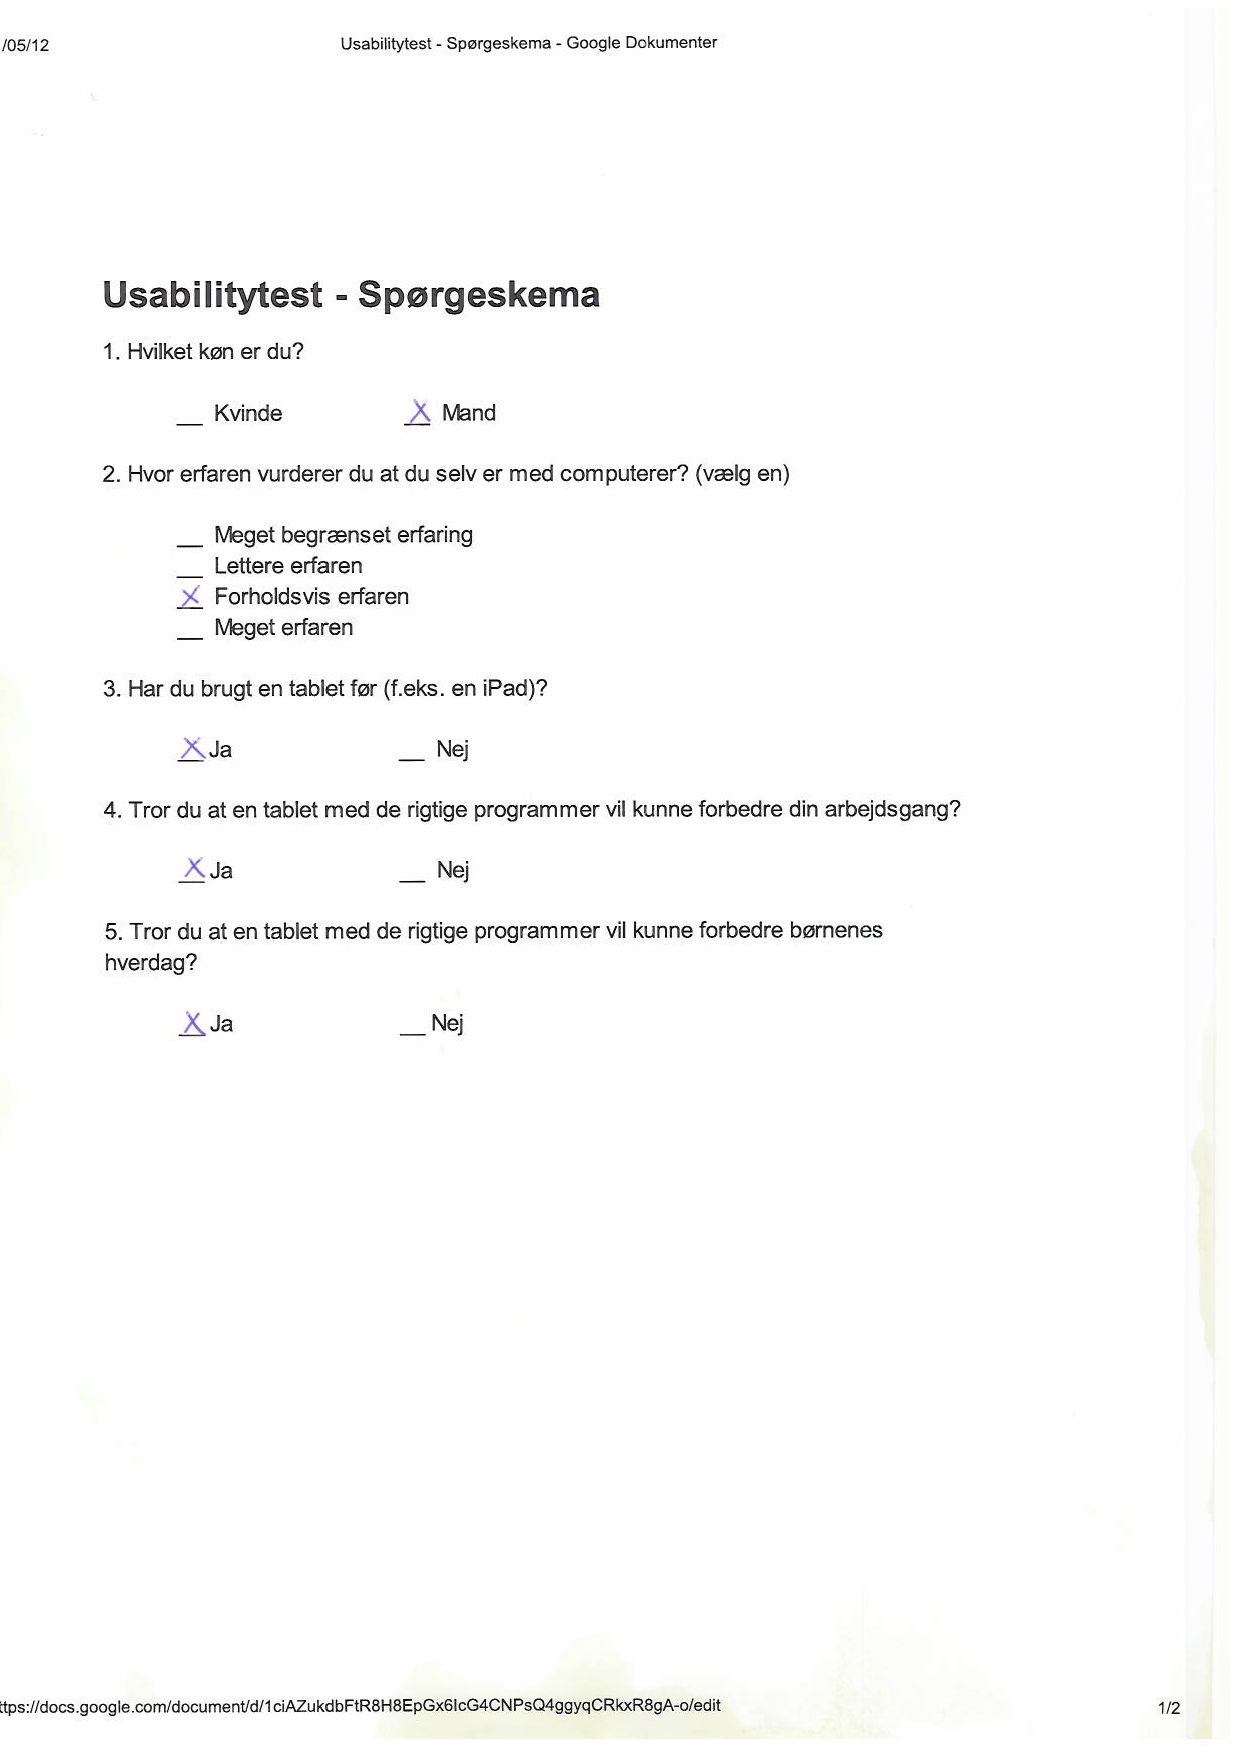
\includegraphics{Appendix/demo_d1.pdf}
	\label{fig:demo_t}
\end{figure}

\begin{figure}[h]
	\centering
		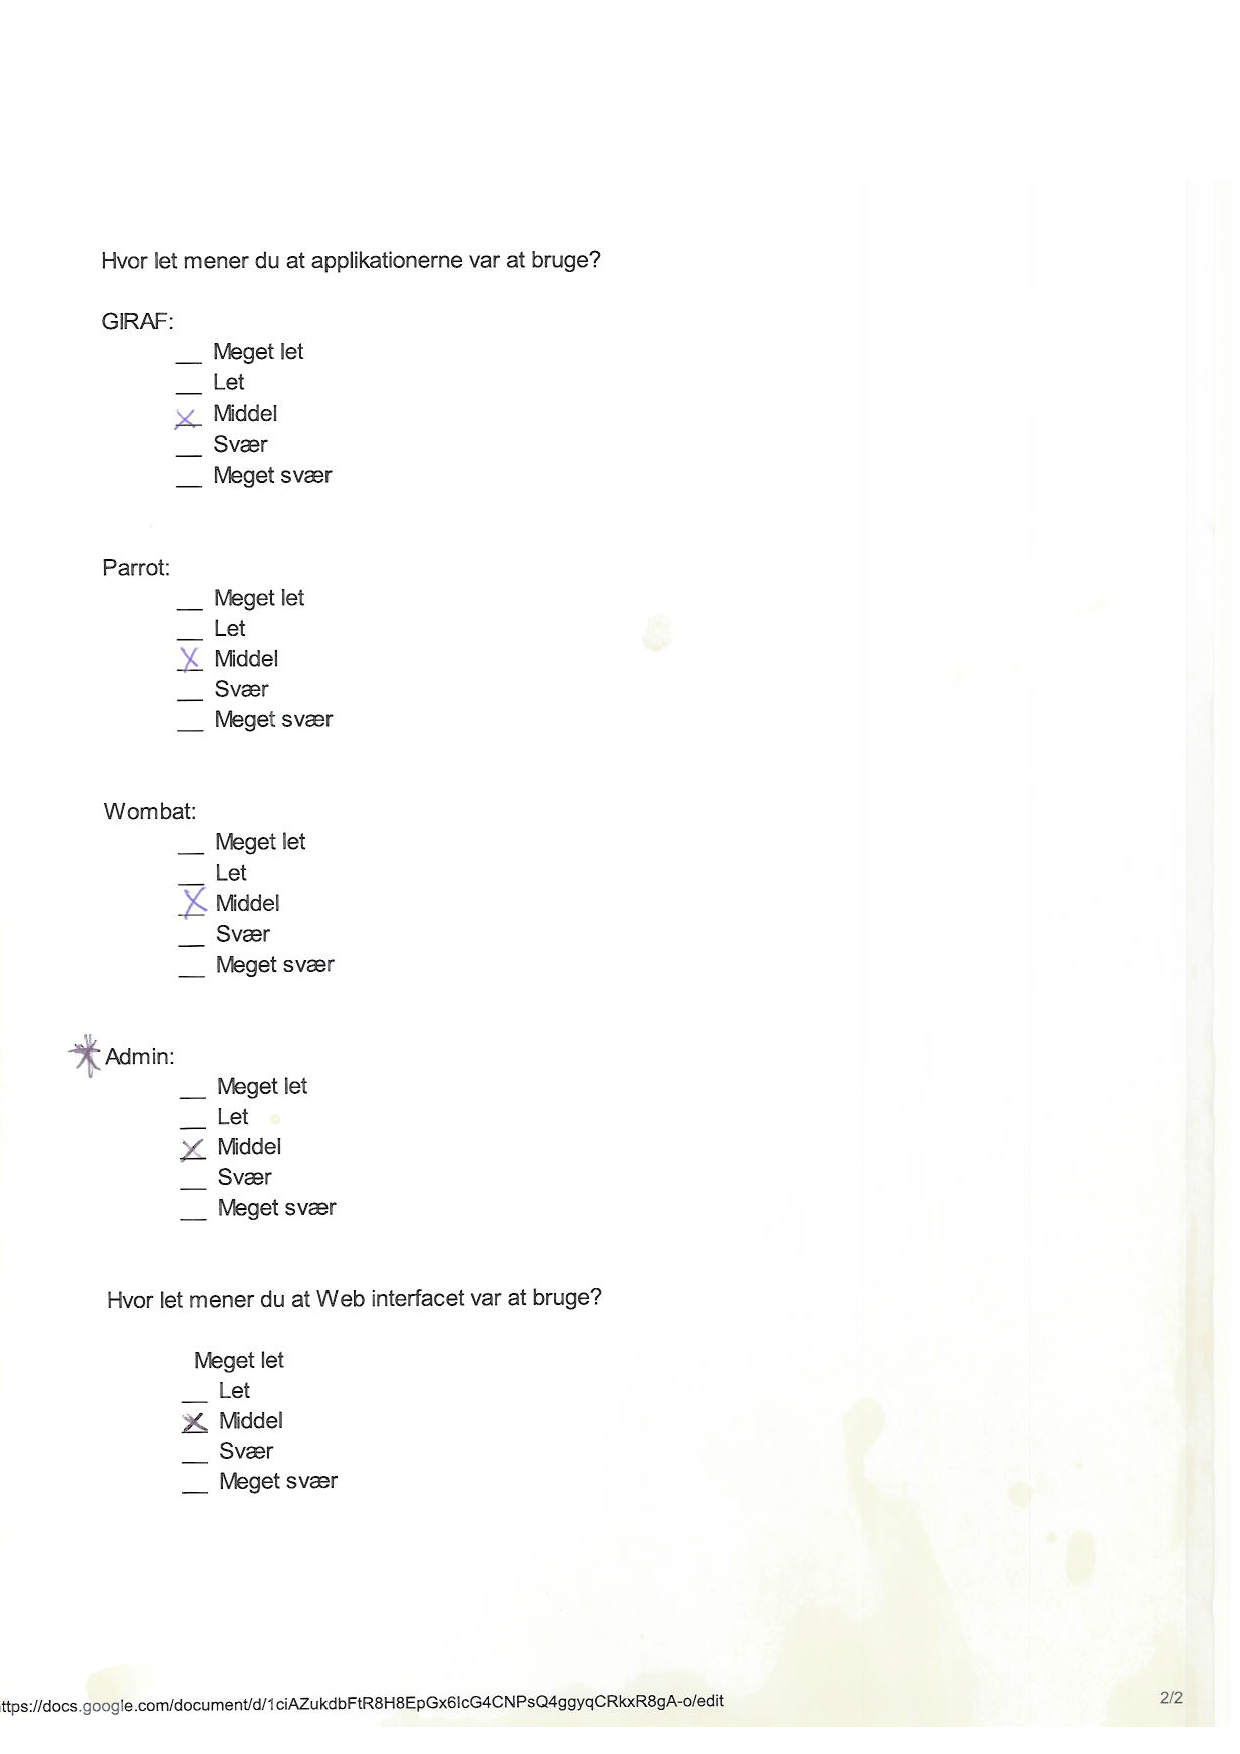
\includegraphics{Appendix/demo_d2.pdf}
	\label{fig:demo_t}
\end{figure}

\begin{figure}[h]
	\centering
		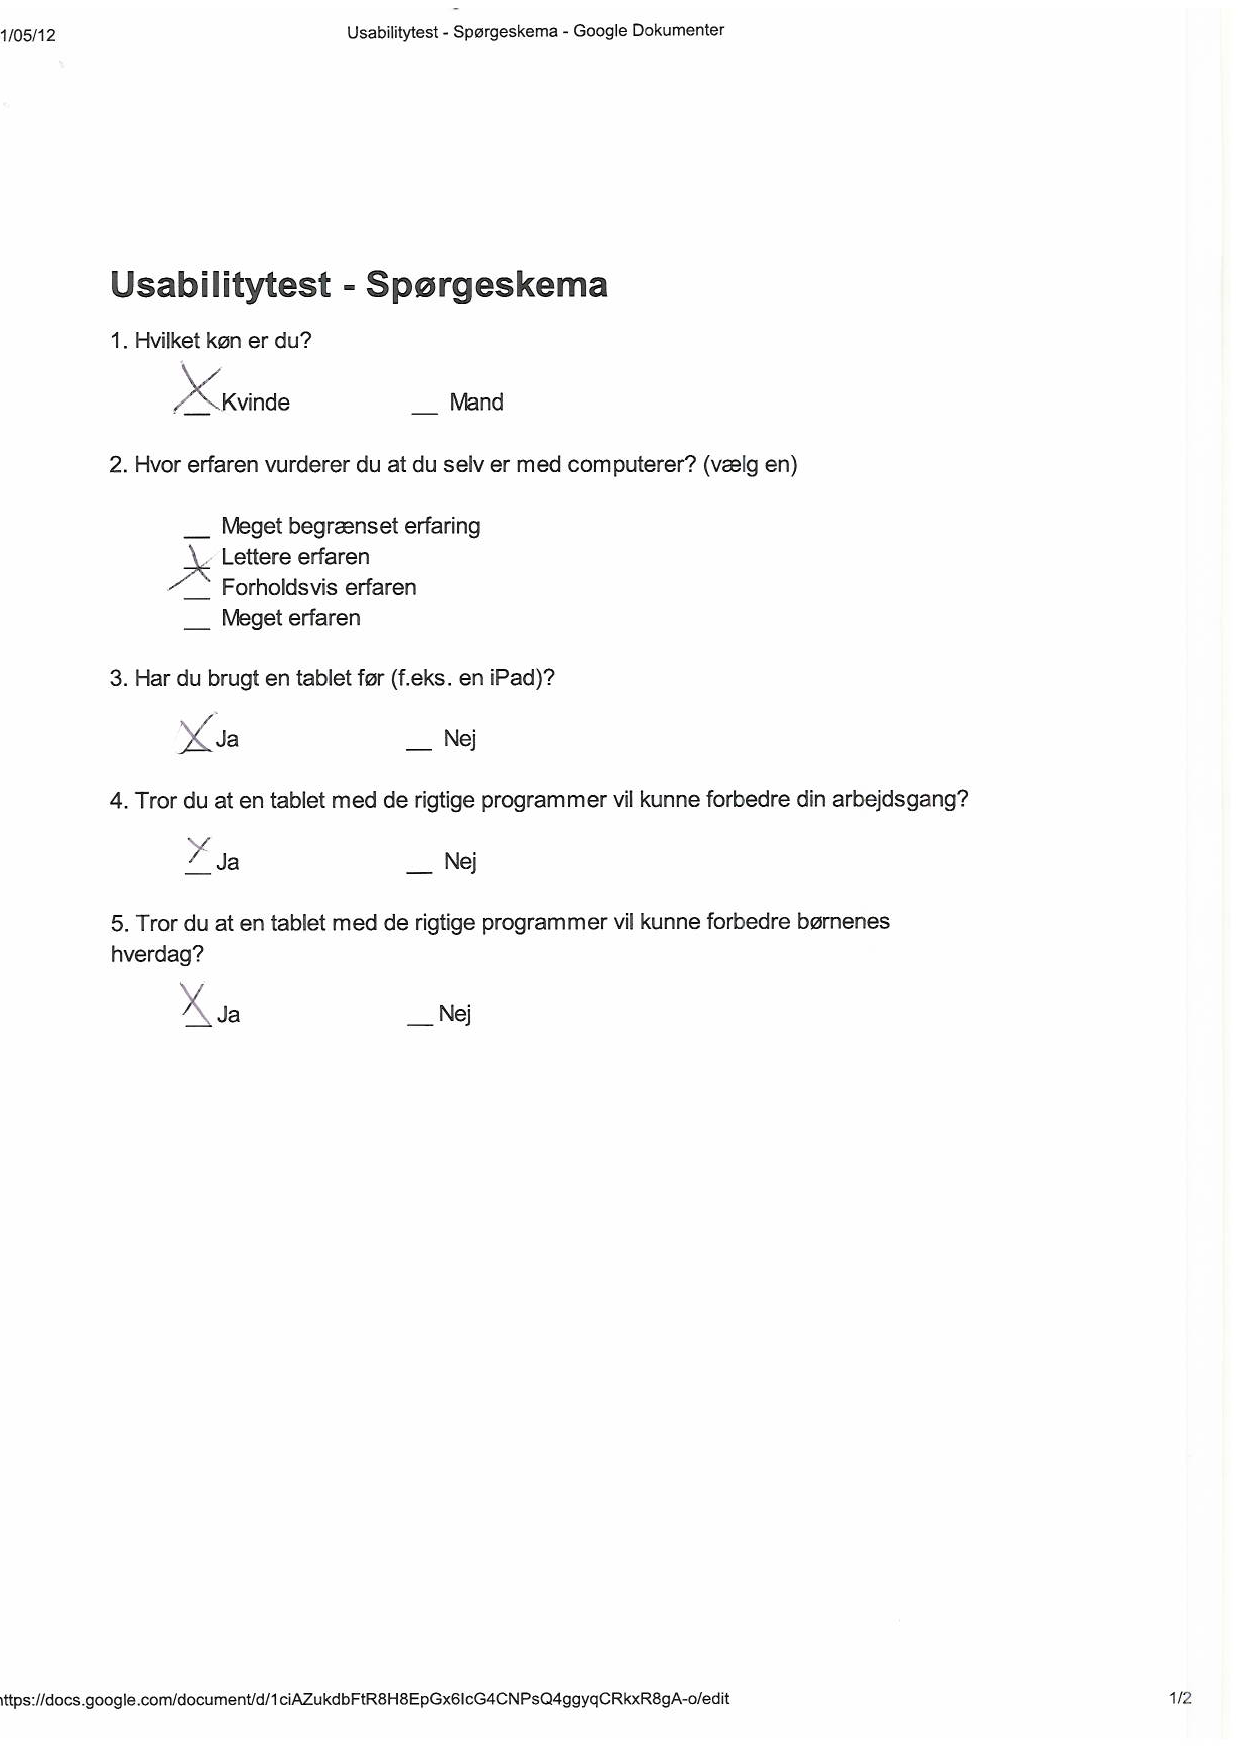
\includegraphics{Appendix/demo_m1.pdf}
	\label{fig:demo_t}
\end{figure}

\begin{figure}[h]
	\centering
		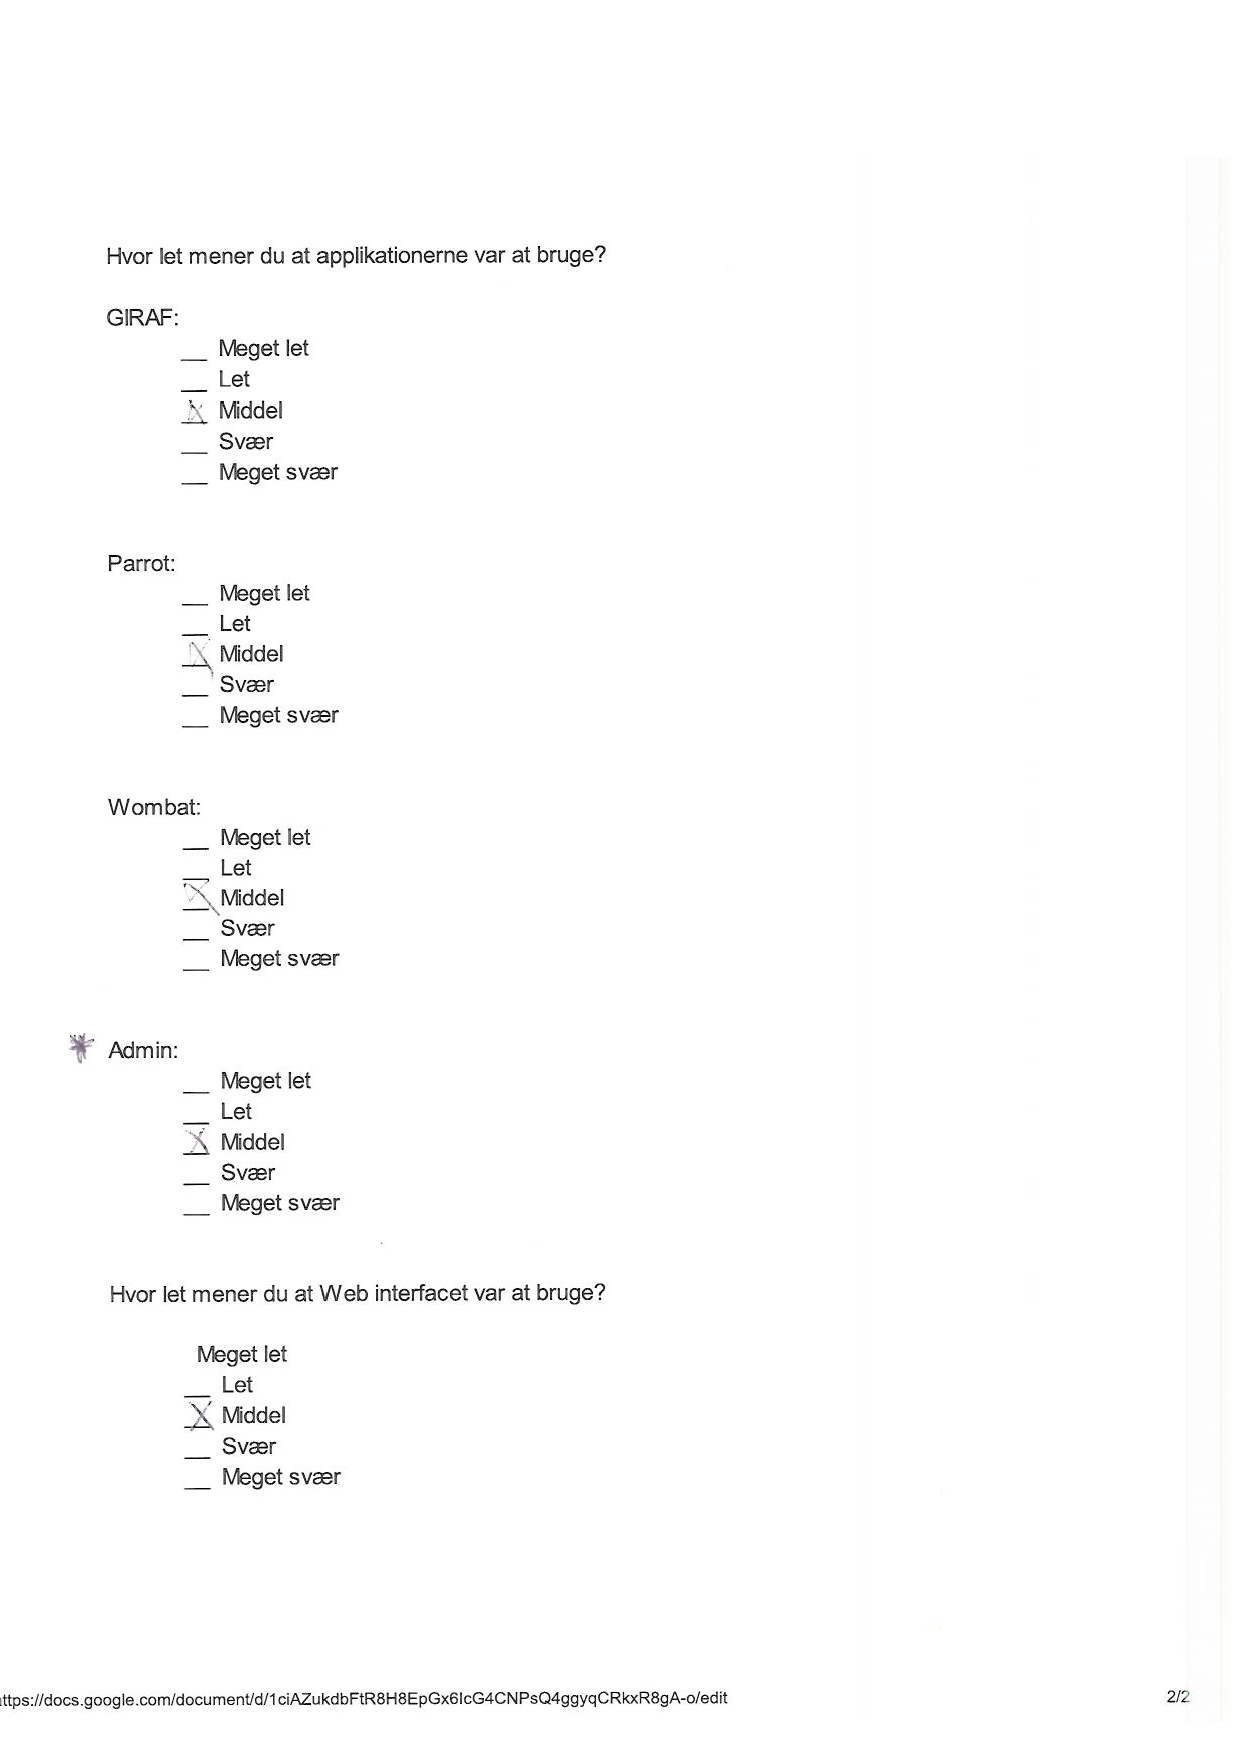
\includegraphics{Appendix/demo_m2.pdf}
	\label{fig:demo_t}
\end{figure}

\begin{figure}[h]
	\centering
		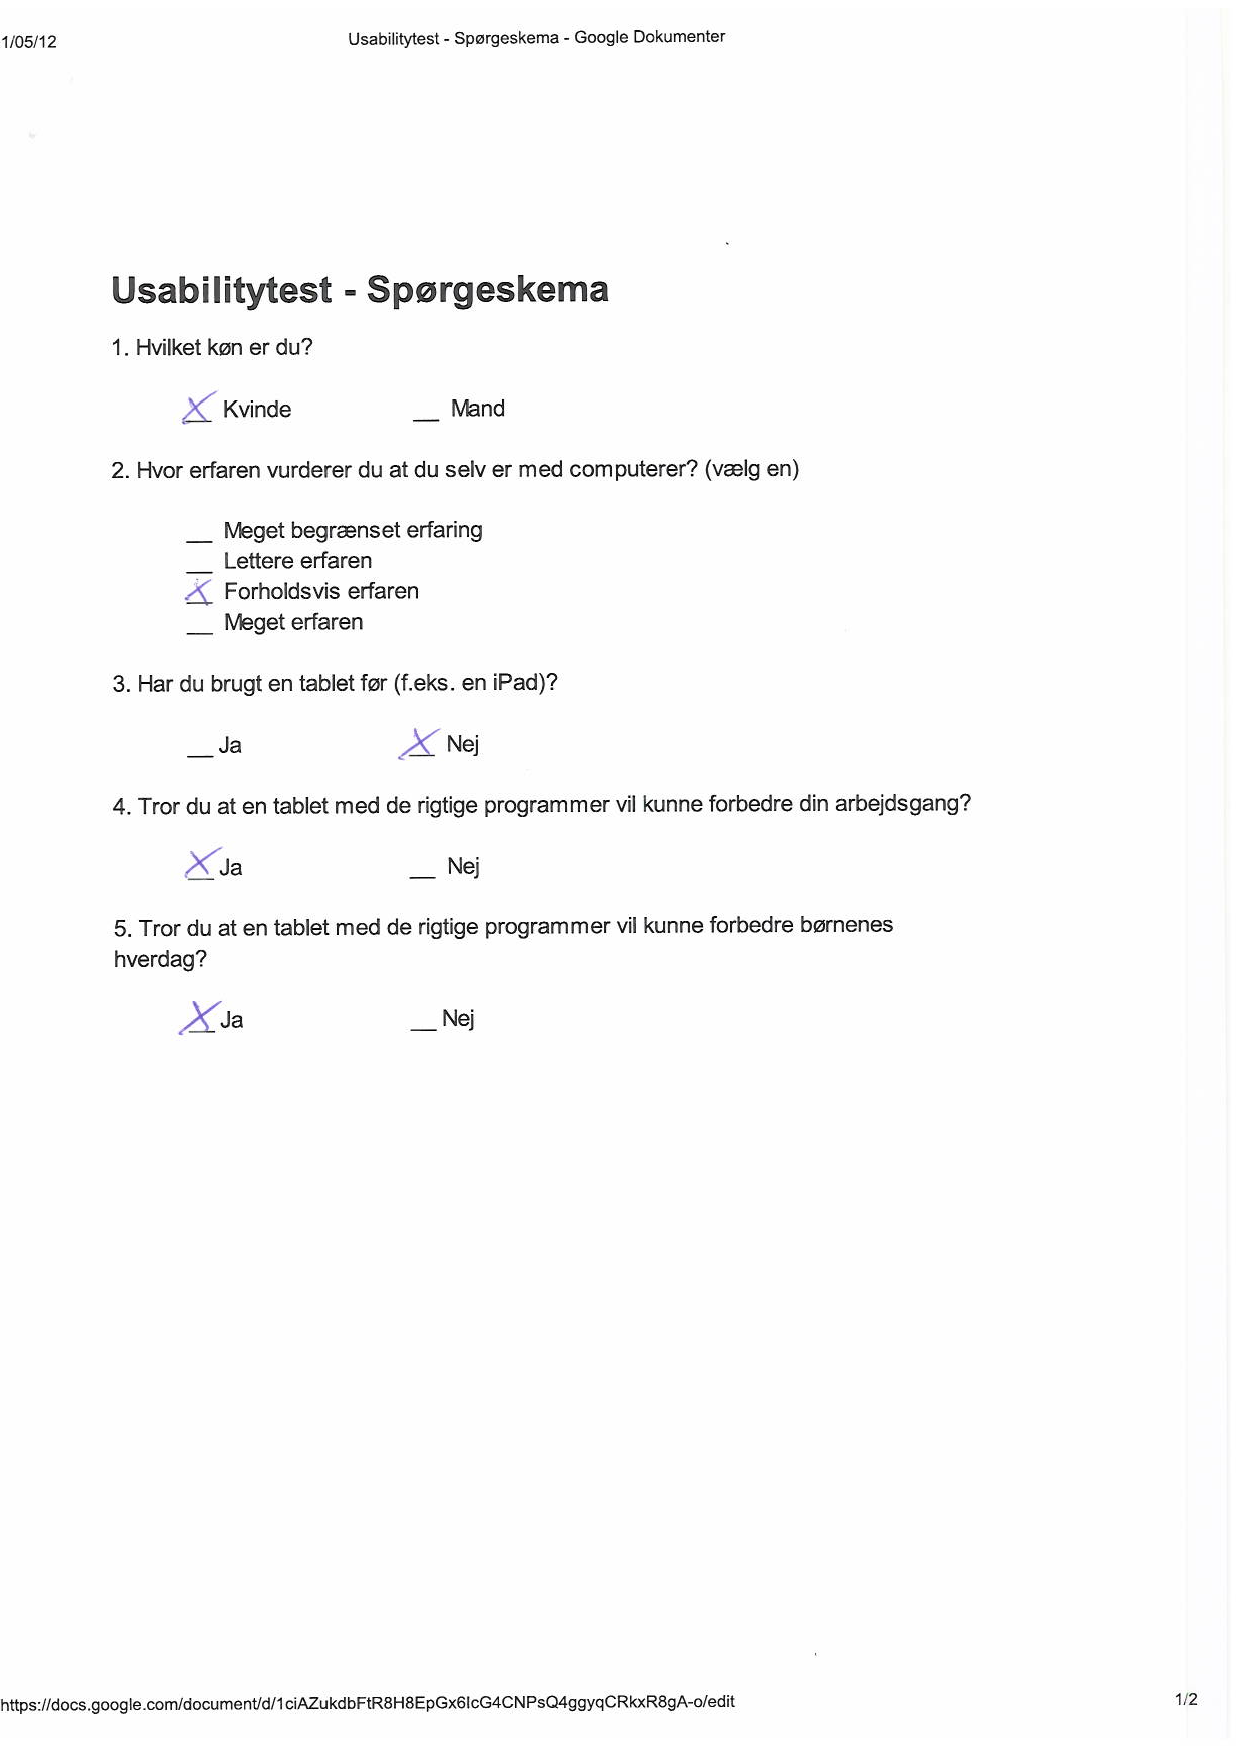
\includegraphics{Appendix/demo_t1.pdf}
	\label{fig:demo_t}
\end{figure}

\begin{figure}[h]
	\centering
		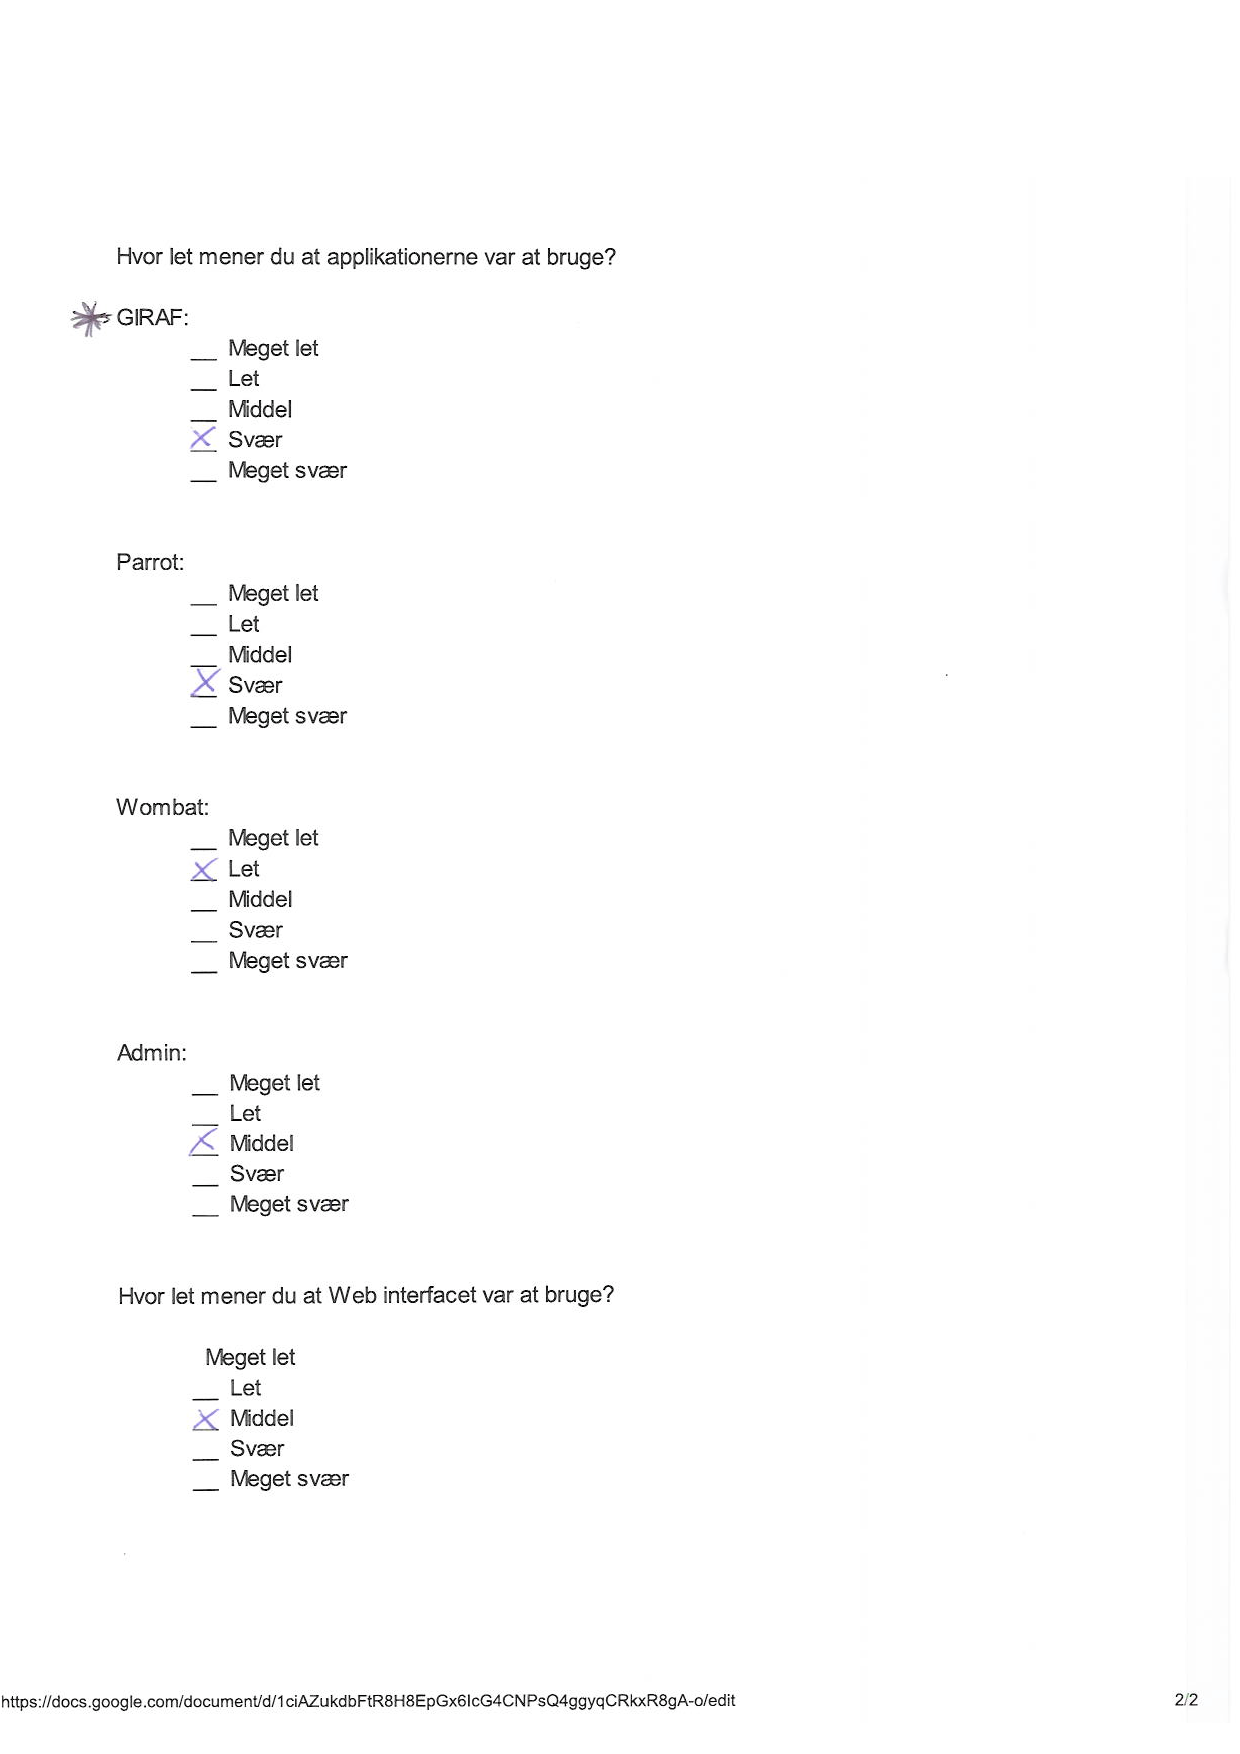
\includegraphics{Appendix/demo_t2.pdf}
	\label{fig:demo_t}
\end{figure}

\begin{figure}[h]
	\centering
		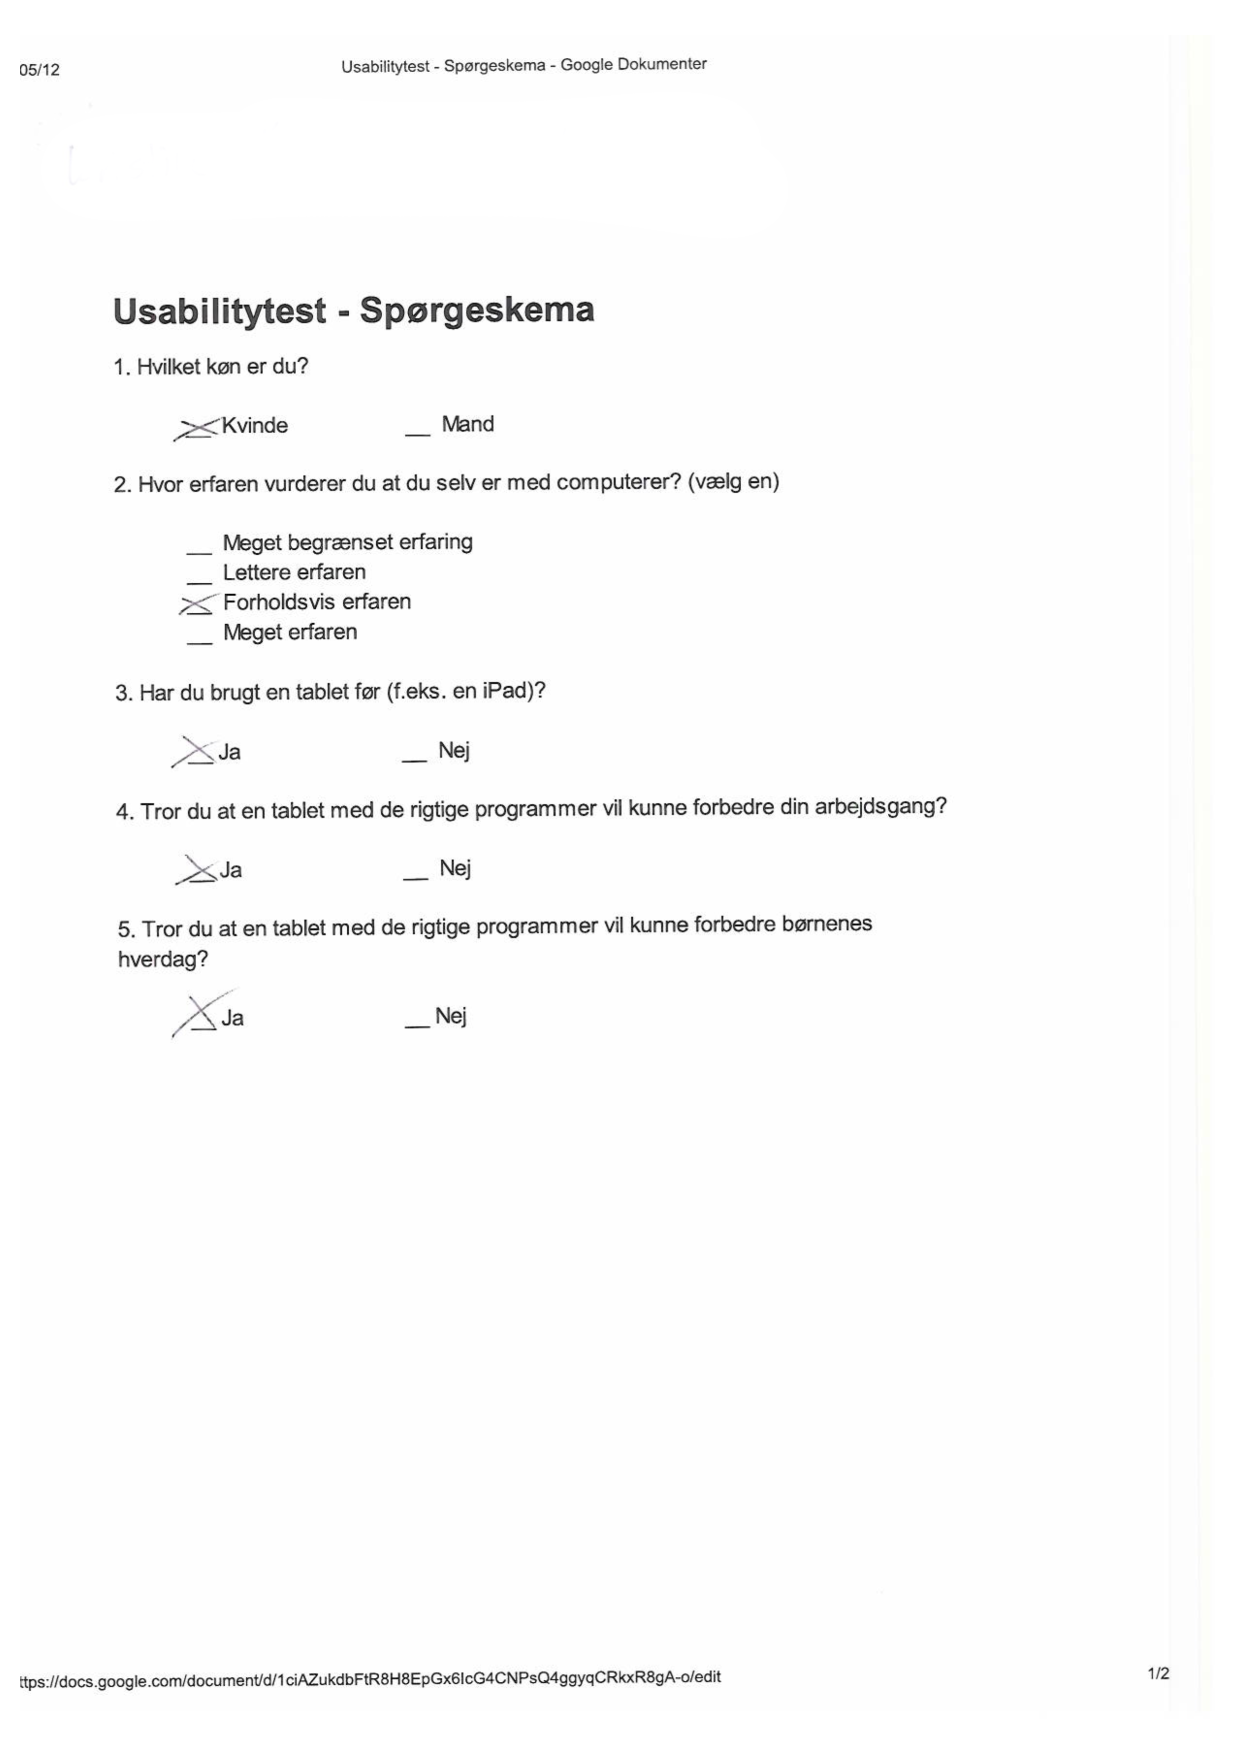
\includegraphics{Appendix/demo_k1.pdf}
	\label{fig:demo_t}
\end{figure}

\begin{figure}[h]
	\centering
		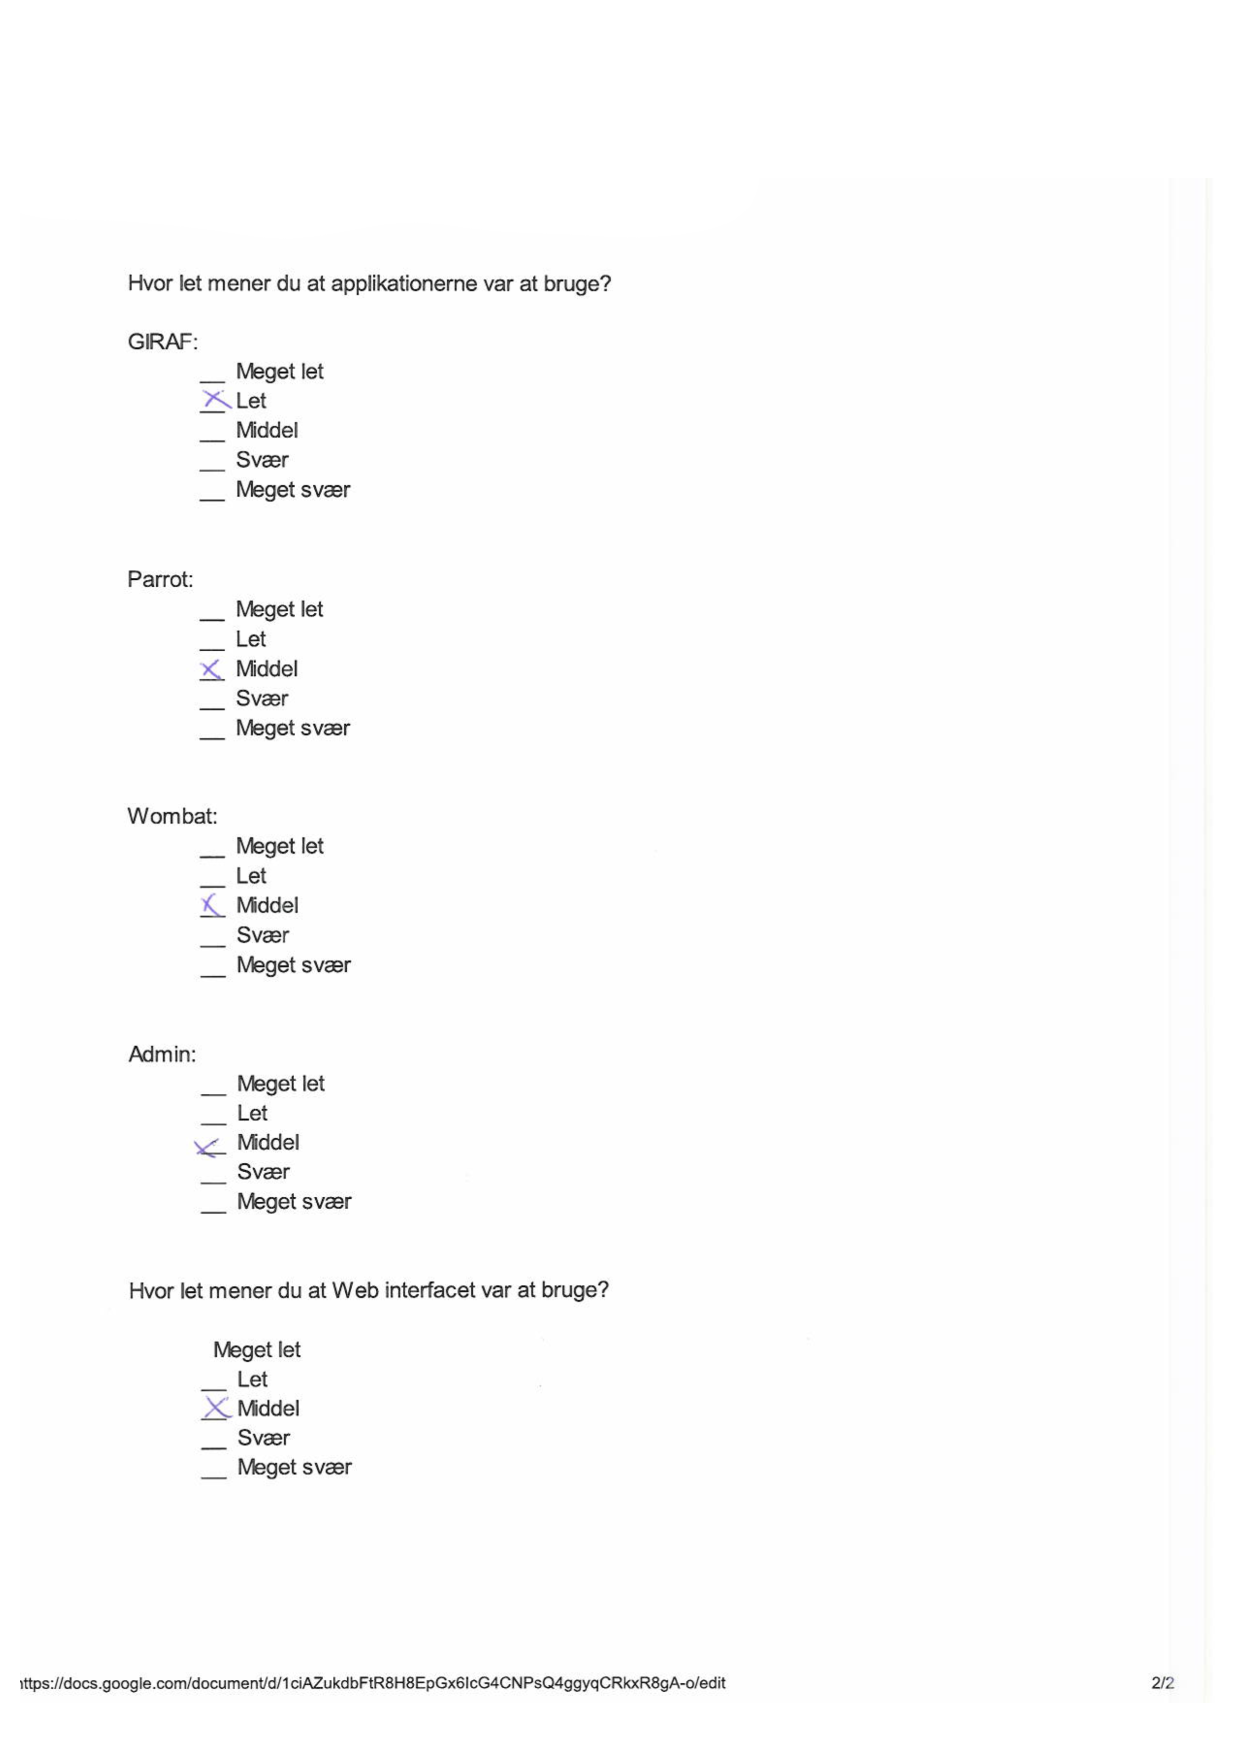
\includegraphics{Appendix/demo_k2.pdf}
	\label{fig:demo_t}
\end{figure}

\begin{figure}[h]
	\centering
		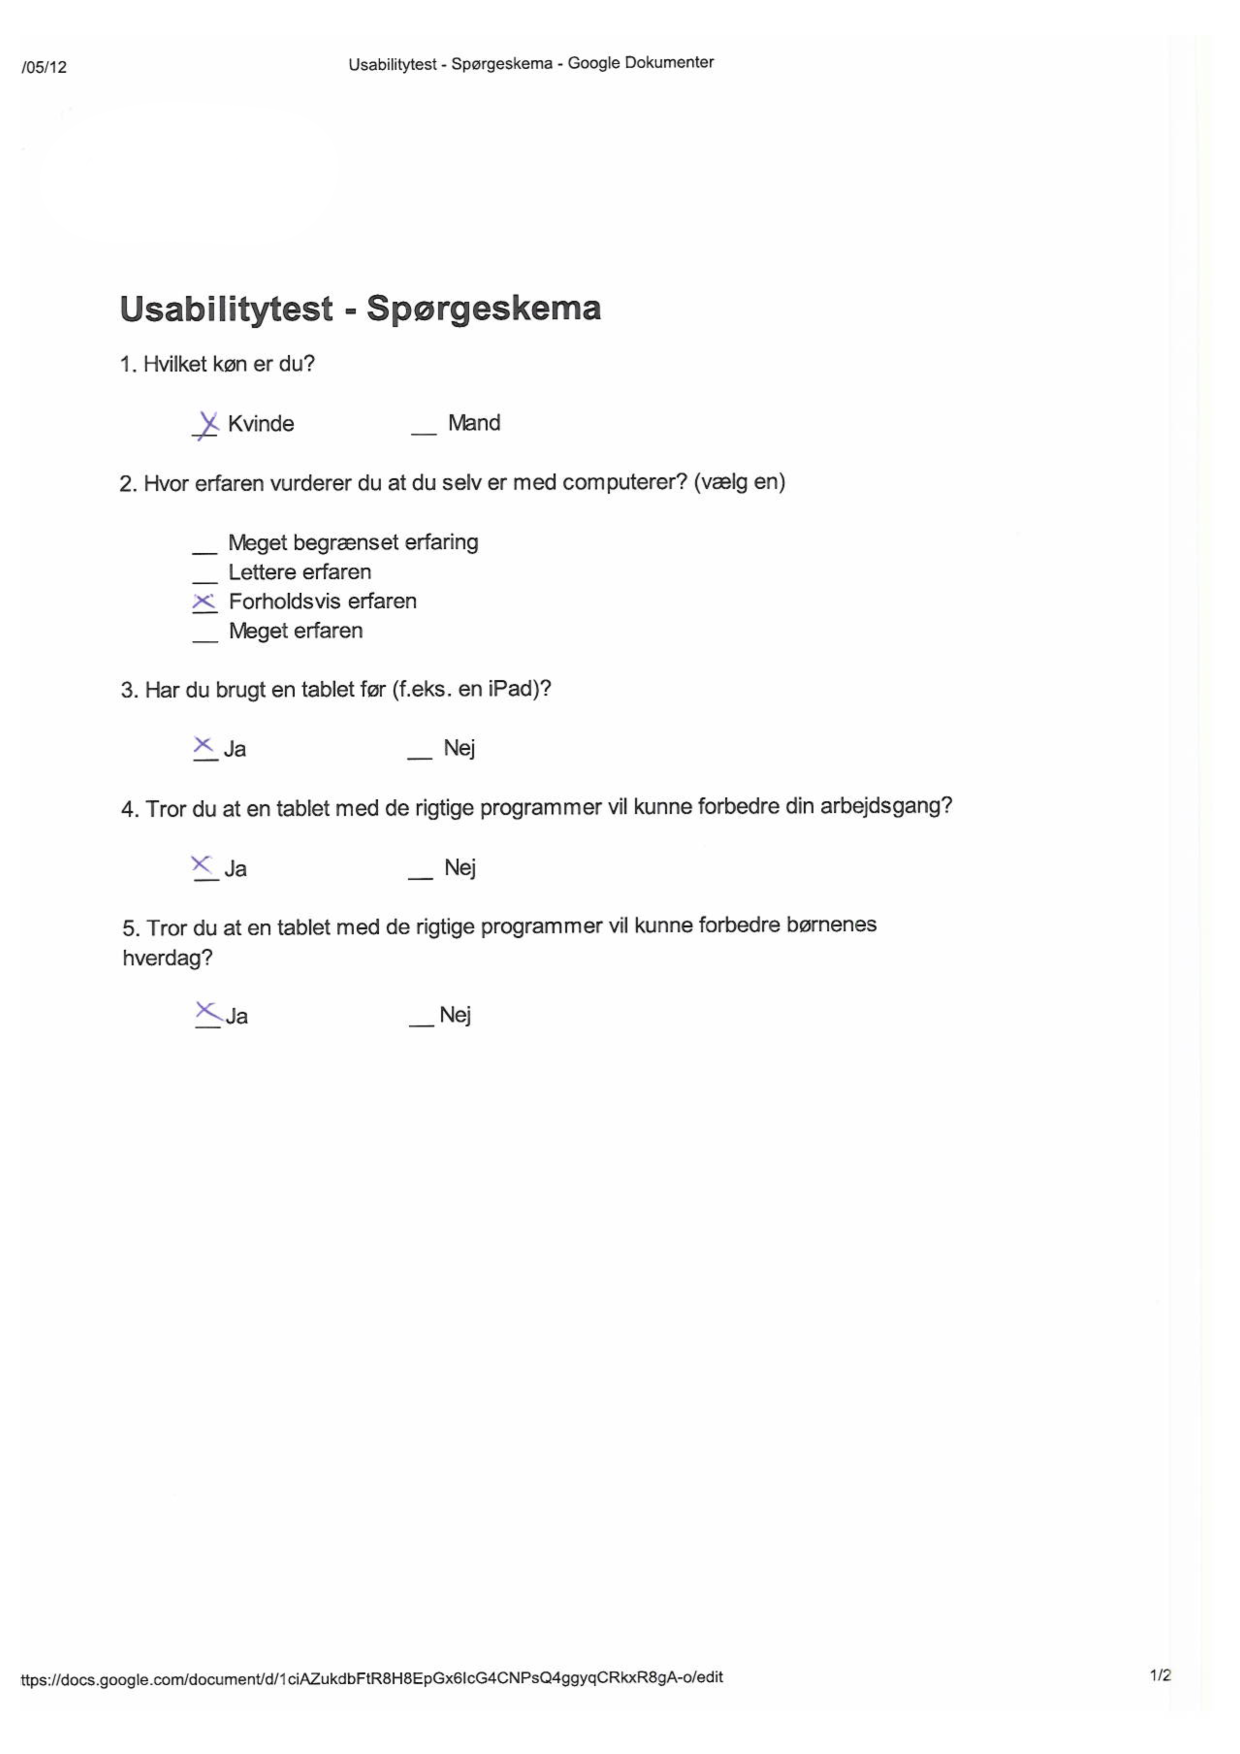
\includegraphics{Appendix/demo_ma1.pdf}
	\label{fig:demo_t}
\end{figure}

\begin{figure}[h]
	\centering
		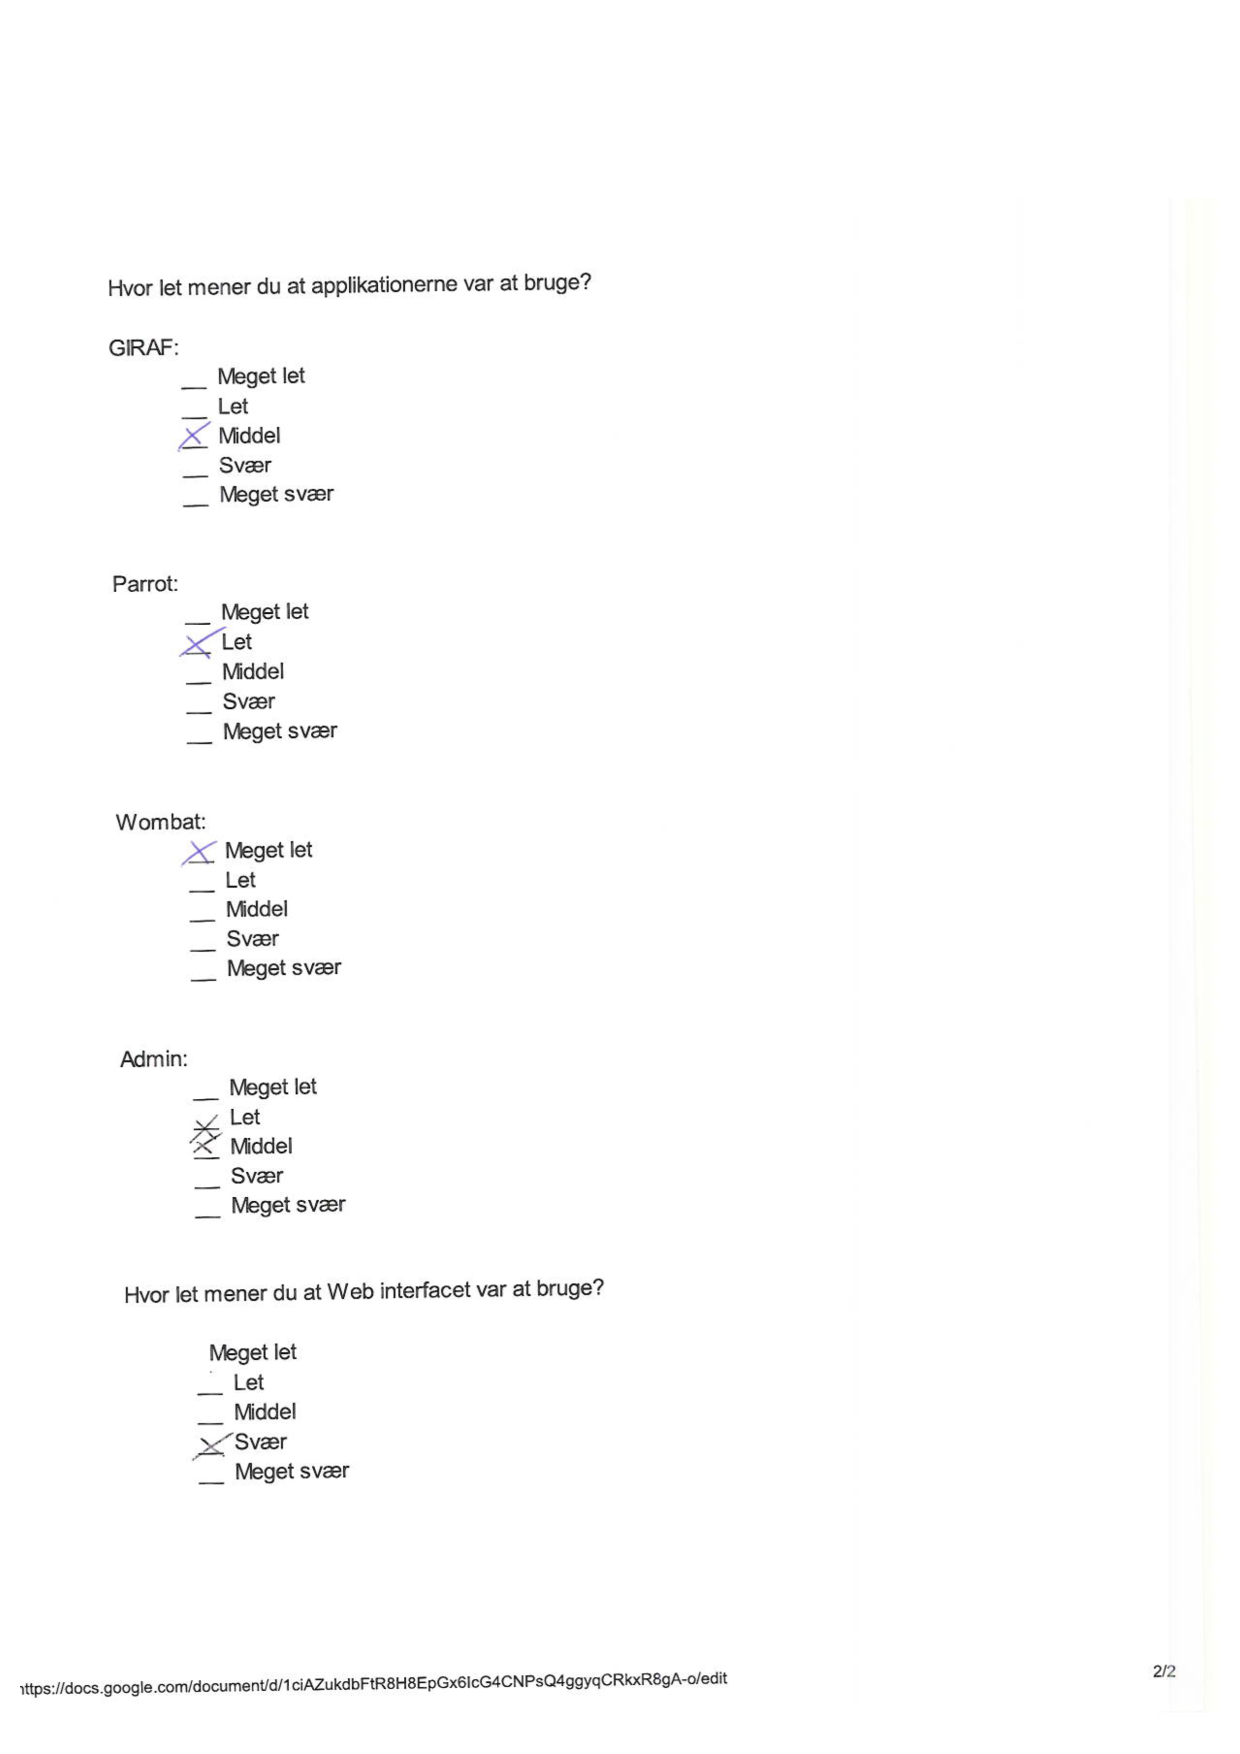
\includegraphics{Appendix/demo_ma2.pdf}
	\label{fig:demo_t}
\end{figure}

\section{Usability Assignments}
\label{sec:usabilityAss}
Admin applikation er en applikation der skal bruges til at styre informationer fra hver enkelt institution. Dette kan g\o{}re ved at manipulere data omkring institutioner og brugere.

Usability Opgaver:
\begin{itemize}
\item Opret en ny barne profil med f\o{}lgende informationer:
\begin{itemize}
		\item navn: 			Thomas Thomasen
	\item telefonnummer: 	12345678
		\item Afdeling:		Myretuen
		\end{itemize}
\item F\aa{} vist den nu oprettede barne profils informationer.
\item Find min profil og rediger navnet p\aa{} profilen fra Tony Stark til dit eget navn.
\item Tilf\o{}j den nu oprettede Thomas Thomasen til mine b\o{}rn.
\item Tilf\o{}j Applikationerne Wombat og Parrot til barnet Thomas Thomasen.
\item Fjern Thomas Thomasen fra afdelingen Myretuen.
\item Tilf\o{}j Thomas Thomasen til afdelingen Bikuben.
\end{itemize}

\section{Unit Test Results}
\label{app:unitTestResults}
In this section the results for the remaing unit tests can be found.

\begin{figure}[h]
	\centering
		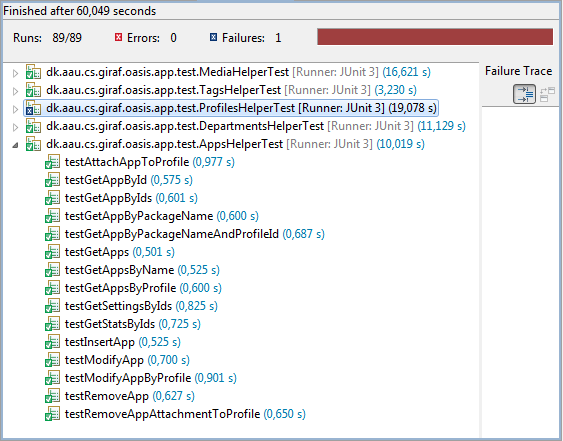
\includegraphics[width=\textwidth]{Images/unit_testing/app_helper_tests.PNG}
	\caption{The result from the \texttt{appsHelper} tests.}
	\label{fig:app_helper_tests}
\end{figure}

\begin{figure}[h]
	\centering
		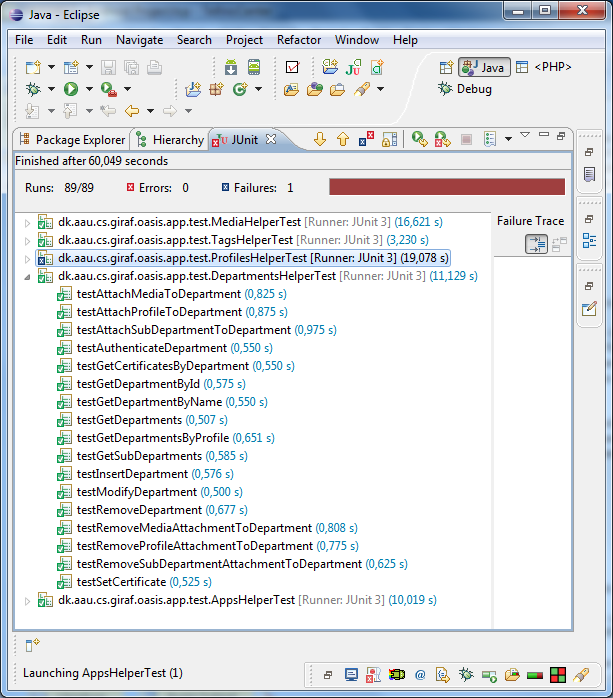
\includegraphics[width=\textwidth]{Images/unit_testing/department_helper_tests.PNG}
	\caption{The result from the \texttt{departmentHelper} tests.}
	\label{fig:department_helper_tests}
\end{figure}

\begin{figure}[h]
	\centering
		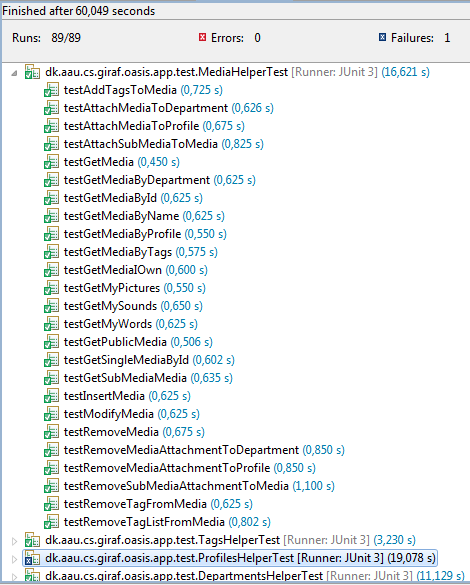
\includegraphics[width=\textwidth]{Images/unit_testing/media_helper_tests.PNG}
	\caption{The result from the \texttt{mediaHelper} tests.}
	\label{fig:media_helper_tests}
\end{figure}

\begin{figure}[h]
	\centering
		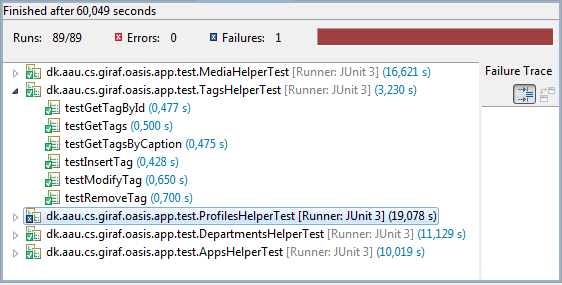
\includegraphics[width=\textwidth]{Images/unit_testing/tag_helper_tests.PNG}
	\caption{The result from the \texttt{tagsHelper} tests.}
	\label{fig:tag_helper_tests}
\end{figure}

% Bibliography.
\addcontentsline{toc}{chapter}{Bibliography}
\bibliographystyle{alpha}
\bibliography{Bibtex/bibliography}
\label{bib}

% A page used to attach the CD-ROM.
\cleardoublepage
\thispagestyle{empty}
\vspace*{4cm}
\label{cd}
{\centering This page is left blank for the purpose of containing the attached CD-ROM.}

\listoffixmes

\end{document}